\documentclass[a4paper,oneside,12pt]{book}

% Variable definitions
\newcommand{\thesistitle}{HubSpot Software Engineering Internship} % Your thesis title, this is used in the title and abstract
\newcommand{\degree}{MAI (Computer Engineering)} % Your degree name, this is used in the title page and abstract
\newcommand{\typeofthesis}{Internship Report} % dissertation, Final Year Project, report, etc.
\newcommand{\authorname}{Stefano Lupo} % Your name, this is used in the title page and PDF stuff
\newcommand{\authorid}{14334933} % Your ID
\newcommand{\keywords}{HubSpot, Software Engineering, Programming, Computer Engineering, 4E4 Internship} % Keywords for your thesis
\newcommand{\school}{\href{http://www.scss.tcd.ie}{School of Computer Science and Statistics}} % title page

\title{\thesistitle}
\author{\authorname}

% Configure output pdf properties
\AtBeginDocument{
\hypersetup{pdftitle=\thesistitle}
\hypersetup{pdfauthor=\authorname}
\hypersetup{pdfkeywords=\keywords}
\hypersetup{pdfsubject=\degree}
}

% Language and font encodings
\usepackage[T1]{fontenc} 
\usepackage[utf8]{inputenc}
\usepackage[english]{babel}

% Bibliographical stuff
\usepackage[round,sort,comma,numbers]{natbib}

% Document size
% include showframe as an option if you want to see the boxes
\usepackage[a4paper,top=2.54cm,bottom=2.54cm,left=2.54cm,right=2.54cm,headheight=16pt]{geometry}
\pagestyle{plain} % Embrace simplicity!

% Useful packages
\usepackage{amsmath}
\usepackage[autostyle=true]{csquotes} % Required to generate language-dependent quotes in the bibliography
\usepackage[pdftex]{graphicx}
\graphicspath{{./assets/}}
\usepackage[colorinlistoftodos]{todonotes}
\usepackage[colorlinks=true, allcolors=black]{hyperref}
\usepackage{caption} % if no caption, no colon
\usepackage{sfmath} %use sans-serif in the maths sections too
\usepackage[parfill]{parskip}    % Begin paragraphs with an empty line rather than an indent
\usepackage{setspace} % to permit one-and-a-half or double spacing
\usepackage{enumerate} % fancy enumerations like (i) (ii) or (a) (b) and suchlike
\usepackage{booktabs} % To thicken table lines
\usepackage{fancyhdr}

%%%%%%%%%%%%%%%%%%%%%%%%%%%%%%%%%%%%%%%%%%%%%%%%%%%%%%%%%%%%%%%%%%%%%%%%
% My Packages
%%%%%%%%%%%%%%%%%%%%%%%%%%%%%%%%%%%%%%%%%%%%%%%%%%%%%%%%%%%%%%%%%%%%%%%%
\usepackage{enumitem} % Nested lists a la TOC (plan)
\setlist[enumerate]{label*=\arabic*.}

\usepackage{scrextend}  % List with description all descriptions tabbed as wide as longest
\addtokomafont{labelinglabel}{\itshape} % Who knows what this does

\usepackage{listings} % Code listing
\definecolor{dkgreen}{rgb}{0,0.6,0}
\lstdefinestyle{javaStyle} {
  language=Java,
  aboveskip=5mm,
  belowskip=5mm,
  showstringspaces=false,
  columns=flexible,
  basicstyle={\footnotesize\ttfamily},
  numberstyle={\tiny},
  numbers=left,
  keywordstyle=\color{blue},
  commentstyle=\color{dkgreen},
  stringstyle=\color{purple},
  breaklines=true,
  breakatwhitespace=true,
  tabsize=1,
  captionpos=b,
  morekeywords={@Inject, {@Value.Immutable}, @Override}
}

\lstdefinestyle{protoStyle} {
  aboveskip=5mm,
  belowskip=5mm,
  showstringspaces=false,
  columns=flexible,
  basicstyle={\footnotesize\ttfamily},
  numberstyle={\tiny},
  numbers=left,
  keywordstyle=\color{blue},
  commentstyle=\color{dkgreen},
  stringstyle=\color{purple},
  breaklines=true,
  breakatwhitespace=true,
  tabsize=1,
  morekeywords={optional, required, message, enum, repeated},
  captionpos=b
}

\usepackage{float} % Figure placement

\usepackage{xcolor}

\usepackage[toc,page]{appendix}
\renewcommand{\appendixname}{Annex}
%%%%%%%%%%%%%%%%%%%%%%%%%%%%%%%%%%%%%%%%%%%%%%%%%%%%%%%%%%%%%%%%%%%%%%%%

%%%%%%%%%%%%%%%%%%%%%%%%%%%%%%%%%%%%%%%%%%%%%%%%%%%%%%%%%%%%%%%%%%%%%%%
% Custom commands
%%%%%%%%%%%%%%%%%%%%%%%%%%%%%%%%%%%%%%%%%%%%%%%%%%%%%%%%%%%%%%%%%%%%%%%%
\newcommand{\team}{Email Sending Infrastructure}
\newcommand{\sneaktitle}[1]{\hfill\break\break\textbf{#1}\hfill\break}
\newcommand{\refcode}[1]{code listing \ref{#1}}
\newcommand{\refsec}[1]{section \ref{#1}}
\newcommand{\refeq}[1]{equation \ref{#1}}
\newcommand{\reftbl}[1]{table \ref{#1}}
\newcommand{\reffig}[1]{figure \ref{#1}}
\newcommand{\refapp}[1]{appendix \ref{#1}}
\definecolor{light-gray}{gray}{0.95}
\lstset{language=java, basicstyle={\normalsize\ttfamily\bfseries},}
\newcommand{\java}[1]{\colorbox{light-gray}{\lstinline{#1}}}
\newcommand{\sub}[1]{_\text{#1}}
%%%%%%%%%%%%%%%%%%%%%%%%%%%%%%%%%%%%%%%%%%%%%%%%%%%%%%%%%%%%%%%%%%%%%%%%


% Default to Sans-Serif
\renewcommand{\familydefault}{\sfdefault}

% Options: Sans-Serif, Computer Modern(latex default), palatino
\usepackage{mathpazo} % math fonts
\usepackage{palatino} % nicer font

% Use continuous equation numbers
\renewcommand{\theequation}{\arabic{equation}} 

% Format Chapter headings appropriately
\usepackage{titlesec}
\titleformat{\chapter}[block] 
{\normalfont\huge\bfseries}{\thechapter}{0.6cm}{} 

% Format Section headings appropriately
\titleformat{\section}[block] 
{\normalfont\Large\bfseries}{\thesection}{0.6cm}{} 

% Format SubSection headings appropriately
\titleformat{\subsection}[block] 
{\normalfont\large\bfseries}{\thesubsection}{0.6cm}{} 

% Update Code Listings
\renewcommand{\lstlistingname}{Code Listing}% Listing -> Code Listing
\renewcommand{\lstlistlistingname}{List of \lstlistingname s}% List of Listings -> List of Code Listings

\frontmatter
\begin{document}
\begin{titlepage}

\center % Center everything on the page

%% All the text parameters should be taken from the start of the main.tex file.
%% You should only alter stuff here if you want to change the layout

%----------------------------------------------------------------------------------------
%	LOGO SECTION
%----------------------------------------------------------------------------------------
%% Choose one of the following -- a colour or black-and-white logo


\includegraphics{assets/Trinity_RGB_transparent_main.png}\\[1cm] 
%\includegraphics[width=12cm]{title/black-stacked-trinity.jpg}\\[1cm] 

\Large \school\\[1.5cm] % Minor heading such as course title
\ifdefined\department
\large \department\\[1.5cm] % Minor heading such as course title
\fi

%----------------------------------------------------------------------------------------
%	TITLE SECTION
%----------------------------------------------------------------------------------------
\makeatletter
{ \huge \bfseries \thesistitle}\\[1.5cm] % Title of your document
 

%----------------------------------------------------------------------------------------
%	AUTHOR SECTION
%----------------------------------------------------------------------------------------

\ifdefined\authorid
\authorname\\ % Your name
\authorid\\[2cm] % Your Student ID
\else
\authorname\\[2cm] % Your name
\fi

%----------------------------------------------------------------------------------------
%	DATE SECTION
%----------------------------------------------------------------------------------------

{\large \today}\\[2cm] % Date, change the \today to a set date if you want to be precise

 
%----------------------------------------------------------------------------------------
%	TYPE OF THESIS SECTION
%----------------------------------------------------------------------------------------
 An \typeofthesis\ submitted in partial fulfillment\\of the requirements for the degree of\\
\degree

\vfill % Fill the rest of the page with whitespace

\end{titlepage}

\pagenumbering{roman}


\mainmatter
\section*{\Huge{Declaration}}
\vspace{1cm}
I hereby declare that this project is entirely my own work and that it has not been submitted as an exercise for a degree at this or any other university.

\vspace{1cm}
I have read and I understand the plagiarism provisions in the General Regulations of the University Calendar for the current year, found at \url{http://www.tcd.ie/calendar}.
\vspace{1cm}

I have also completed the Online Tutorial on avoiding plagiarism `Ready Steady Write', located at
\url{http://tcd-ie.libguides.com/plagiarism/ready-steady-write}.
\vspace{3cm}

Signed:~\rule{5cm}{0.3pt}\hfill Date:~\rule{5cm}{0.3pt}

\newpage
\onehalfspacing
\raggedright %\raggedright turns off justification and hyphenation

\section*{\Huge{Acknowledgements}}

\tableofcontents
\listoffigures
\listoftables
\lstlistoflistings
\newpage


\section*{\Huge{Nomenclature}}
\begin{tabular}{lp{15cm}l}
    $NDN$ & Named Data Networking \\
    $CCN$ & Content Centric Networking \\
    $LSR$ & Link State Routing \\
    $NLSR$ & NDN Link State Routing \\
\end{tabular}
\vspace{2cm)
 % Need to uncomment stuff in here..

\chapter{Introduction}

\section{What is HubSpot?}
\textit{"HubSpot is inbound marketing and sales software that helps companies attract visitors, convert leads, and close customers."} \cite{whatIsHubSpot}\hfill\break

Over the past few decades, there has been a monumental shift in how consumers think about, shop for and purchase products. Consumers are now far more skeptical towards traditional marketing campaigns, for example via TV or print advertisements. Thanks to the near endless amount of information available on the internet, consumers are much more informed about the products or services they are purchasing and place their trust in credible third party reviews. In response to the modern consumer, a modern marketing strategy must be put in place. 

HubSpot is built with one core belief in mind - \textit{inbound marketing}. Inbound marketing is a strategy in which potential customers are \textit{attracted} to a website (or other establishment) naturally, prior to attempting to convert them into buying customers. The key concept here is that customers must be able to obtain something of value prior to making a purchase. This attracts potential customers to the website, provides them with something they need and gives them an insight into the quality of the product or service on offer. For example, a website of a company selling musical instruments may write a blog post detailing what one should look for when purchasing their first guitar. For a modern consumer looking to purchase a guitar for the first time, it is extremely likely that they will look online for some information and a comprehensive guide on what to look for when purchasing a guitar would be the perfect resource. While reading this article, the consumer could be provided with attractive CTAs (call-to-actions) which, for example, bring them to a list of suggested guitars for beginners. Thus, a potential customer has been naturally \textit{attracted} to the company's online store, after acquiring some knowledge on exactly what they are looking for. This is a stark contrast to the traditional approach to marketing in which the potential customer is simply shown an advertisement for a guitar. This overall concept of inbound marketing is succinctly summarized by the inbound marketing ethos - \textit{don't interrupt buyers, attract them} \cite{whatIsHubSpot}.

\section{The HubSpot Platform}
HubSpot offers a comprehensive suite of products to help businesses employ an inbound marketing strategy, all of which are contained within a single platform.

\subsection{Customer Relationship Management (CRM)}
At the core of the HubSpot platform, is the HubSpot CRM. Simply put, a CRM is a single data source consisting of \textbf{all} the data relating to a given customer. For example, it contains simple properties such as their name, age and address, but can also contain (in HubSpot's CRM) more complex information such as their last purchase, the last time they were contacted by a sales rep etc. Almost all of HubSpot's products aim to build \textit{personalized} experiences for their customers and the data required to drive these personalized experiences often comes from the CRM. As a CRM is such an integral part of a modern business' daily operations, HubSpot offers their CRM for free. 

\subsection{Sites}
HubSpot also provides a comprehensive website builder allowing users to build custom websites using a drag-and-drop style editor. This hugely simplifies the process of building a website, requiring zero knowledge of web development. These websites can be fully database driven, allowing the experience to be tailored to individual users. This product also includes a host of tools such as forms, CTAs, blogging and many others. All of the pages will be fully responsive and render perfectly on devices of any screen size. These sites can be hosted with HubSpot, further simplifying the website setup process.

\subsection{Email Marketing}
One of HubSpot's most popular tools is the marketing email product. Marketing emails can be built using an intuitive drag-and-drop editor and can be personalized on a per-subscriber basis, backed by HubSpot's CRM. Emails can be sent to arbitrarily complex subsets of subscribed customers (for example, customers who previously made a purchase, but haven't done so in 6 months). All marketing email that is sent can gather detailed analytics on how subscribers interact with the email, allowing HubSpot's customers to gain a deeper understanding of their customers. Similarly, email content can be optimized using A/B testing backed by machine learned models. A/B testing creates multiple versions of the same email, for example with different fonts and colours. A test send on a small sample of the target subscribers is performed, half of the sample receiving version A and half of the sample receiving version B. Key analytics such as open-rates and click rates are examined in order to attempt to ascertain which email will perform better on average. The better version of the email can then be sent to the remaining subscribers, maximizing the effectiveness of the marketing emails sent.

\subsection{Service Hub}
Modern customer's demand a high level of support should they encounter any issues when using a product or service. Service Hub is a modern tool to enable support staff to provide the high level of customer support that is necessitated today. This product provides a set of tools to enable customers to get in touch with \textit{who} they need to, \textit{when} they need to. It offers a plug and play messaging system for websites, allowing customers to chat with support staff in real time. It also offers a single tool for support staff which consolidates all customer conversations into one place (e.g. emails, support tickets, comments and even some social media support), allowing support staff to easily stay on top of their work. 


\section{The \team{} Team} \label{sec:emailSendingInfra}
The \team{} team is one six teams working on HubSpot's email products. These teams vary in purpose from creating the drag-and-drop email builder, gathering analytics on emails sent, ensuring that no spam email is sent through HubSpot and finally, the \team{} team's purpose, sending the actual final email. Considering the fact that sending email is quite an old and well established mechanism, at first glance, one might wonder why an entire team is needed solely for maintaining the infrastructure for sending the emails. However as HubSpot continues to grow, the number of emails that need to be sent continues to grow. Currently, HubSpot sends upwards of 60 - 70 million marketing emails per day on behalf of their customers. At this scale, sending email becomes a non-trivial task that must be carefully managed, requiring a high emphasis on efficiency at each step. 

There are some major challenges with sending email at this scale, primarily stemming from the fact that SMTP, the Secure Mail Transfer Protocol (see \refsec{sec:smtp}), was developed over 30 years ago. This protocol was designed with (relative to the modern day) very small packet sizes in mind. As such, it is a very \textit{chatty} protocol, requiring several round trips between client and server, which can cause the SMTP conversation required to send even a small email take time on the order of hundreds of milliseconds, or even seconds. Thus, sending millions of emails a day, each taking a (relatively) substantial amount of time, highlights the difficulties faced by the \team{} team. Another challenge of sending email is the variation in recipient servers. Anyone can very easily setup an email server on any machine. As one might expect, attempting to send 100 emails to a small desktop machine on a home network is very different to sending them a high performance mail server in one of Google's data centers. Thus, the \team{} team's systems must be able to handle sending to both types of servers efficiently. 

In today's computing world of multicore processors and high concurrency, the solution to the problem is to asynchronously send the emails, allowing the system to continue to perform useful work while waiting on responses from servers. However as with all concurrent solutions, this adds an extra layer of complexity to the system. System resources, especially the heap, where all of the in-flight emails will be stored, must be carefully managed. Another common issue faced is that recipient servers often apply heavy rate limiting to the IPs sending the emails, or to the SMTP domain from which the email originates. This is done to ensure the recipient servers are not overwhelmed by large spikes of emails from a single domain (a common occurrence when spammers compromise legitimate email accounts). Thus asynchronously sending emails requires distributed rate limiting through distributed semaphores, all of which must be carefully balanced in order to maximize throughput, while maintaining a good relationship with the recipient servers. 

The main project owned by the \team{} team is an internal Mail Transfer Agent (MTA). MTAs are systems responsible for sending email on behalf of clients. This internal MTA began development in 2016 and has been an integral part of HubSpot's email products ever since. The choice to develop an internal MTA may seem odd at first, given that email has been around for decades and many \textit{Mail Transfer Agents as a Service (MTAaaS)} already exist. There were several key reasons for developing an internal MTA. The first was to learn as much information about the email sending process as possible and to relay this information back to HubSpot email marketing customers, allowing them to create the best email marketing campaigns they can. Another key reason is that HubSpot is responsible for sending these marketing emails on behalf of their customers and cannot simply blame a third party should the MTAaaS perform poorly. Finally, it also provides flexibility and allows HubSpot's email products to grow and change overtime as the business dictates.  

The \team{} team is a relatively new team whose main focus is taking ownership of all the code used in HubSpot for the email sending process (including the internal MTA previously discussed). The team saw 25x growth in the number of emails sent through their MTA in 2017 and managed to become \textbf{more} reliable while scaling, enabling HubSpot's email products to grow without constraints.  
\chapter{Team Management and Team Process}
As with any type of team, it is critical that the team is managed appropriately. However, \textit{appropriately} doesn't imply that the team should be managed \textit{strictly}. The \team{} team are a very self-motivated team and thus required no micro management. The day to day managerial tasks fall to the tech-lead (TL). The TL is an experienced engineer who is officially responsible for the success of the team. The TL of \team{} frequently liaises with other teams and senior staff in order to maintain alignment between the goals of the company as a whole and the goals of the team. The \team{} team also recently received a project manager (PM). This role is responsible for working with customers and ensuring the team is prioritizing what will have the most impact on the customers and business as a whole. In the case of the \team{} team, neither the PM nor the TL were concerned with the day-to-day operations of a given engineer on the team. Each of the team members is sufficiently interested and invested in the success of the team that trust is placed in each of the team members to pull their weight. This management strategy aligns directly with HubSpot's ethos of \textit{"use good judgment"}. HubSpot aims to hire the type of employees that can be entirely trusted and believes in letting their employees work in whatever way they are most comfortable, which is typically the way in which they are the most productive.

However, no matter the management style, a solid \textit{team process} is paramount for the success of the team. This involves having well defined methods for managing tasks and monitoring the productivity, morale and competency of the team as a whole. Some of the critical parts of the team process of the \team{} team are outlined in the following sections.

\section{GitHub Enterprise and Issue Tracking}\label{sec:issueTracking}
HubSpot's entire engineering department runs on GitHub Enterprise \cite{githubEnterp}. This is an online platform which provides code hosting, comprehensive version control through Git \cite{git}, tracking issues and managing pull requests. 

A common method of keeping track of what needs to be done inside of a software development team is creating \textit{issues}. An issue is typically a paragraph or two long, outlining a task that the team should work towards to create, fix or improve upon something. A good issue will have context as to \textbf{why} the issue is important, \textbf{who} the issue impacts (negatively or positively) and the overall impact of the issue (for example is it critical or should other more pressing issues be prioritized). 

Internally, HubSpot is a very open company and a lot of teams work very closely together. As such it is perfectly acceptable (and encouraged) that someone from outside of the team create an issue to inform the team of something they think the team should know. Sometimes, the request contained in the issue is actually already in place - for example a request for a feature which already exists. An engineer on the team will typically respond to the issue and can close the issue once a desirable outcome has been reached. 

Critically, issues provided a comprehensive and searchable history of what the team has been working on. Issues often result in a piece of code being (re)written and a pull request submitted. GitHub offers a mechanism for cross referencing issues and pull requests so the issue which incentivized the pull request (and the pull request which resolves the issue) are forever searchable in the Git history of the project. This is extremely useful for engineers who wish to gain some broader context on a piece of the system, allowing them to read the context contained in the pull request and associated issue. 

\section{Task Management}
In order to maximize productivity and maintain a healthy workload, a system must be put in place which dictates how team members are assigned units of work. All units of work were defined in GitHub issues (see \refsec{sec:issueTracking}). The method used by the \team{} team, was to split tasks up into the following five stages:

\begin{labeling}{In-Progress}
	\item [Backlog] This contains tasks which are of low priority and can be deferred until a later date
	\item [Design] This contains tasks which require a considerable amount of planning before being undertaken. Tasks in this stage often result in discussions among the team about how best to tackle the task.
	\item [Ready] Tasks which have enough detail and context that they are ready to be undertaken. More complex tasks that were once in the design category land here once all the corresponding details have been decided upon. These are tasks which engineers on the team should choose as a next task upon completion of a task.
	\item [In-Progress] This contains tasks which are currently being worked on (usually) by a single engineer.
	\item [Completed] Tasks which have been completed this week.
\end{labeling}

All of the tasks are managed through an online platform called Waffle \cite{waffle} which presents a \textit{"Waffle Board"} which displays the tasks in each of the above stages. The team concludes each week with a meeting in which the board is inspected and tasks are moved to new stages as appropriate. This provides a great mechanism for monitoring the team's productivity and ensuring that the team is focused on the most important tasks. 

\section{Communication}
The main method for communication among employees in HubSpot is through Slack \cite{slack}. Slack is a messaging platform which allows users to create and join channels. At HubSpot, most teams have a well-known channel in which all members of the team are present in. People with questions or comments can simply join the Slack channel and send a message. Slack channels and messages are well indexed allowing users to search by keyword to find what they are looking for. This is extremely useful for looking for answers to questions that have likely been answered before, or to find the appropriate Slack channel to ask a question in.

HubSpot also has a number of channels in which engineers can ask for help. For example there is a channel specifically for Java questions where Java experts and beginners can help one and other out. These Slack channels are also very useful to follow in order to pick up random pieces of information. Often times, questions that are asked stimulate interesting conversations, allowing engineers to gain a deeper insight into what was initially asked.

\section{Proactive Operations Reviews}
Operations Reviews (Ops Reviews for short) are meetings in which the health of the system over the past time period is examined. For the \team{} team, these are conducted weekly. HubSpot has a PagerDuty service which allows alerts to be set up based on the system's current health. If one of these alerts triggers, the on-call engineer on the team receives a notification informing them of the alert. These are critical alerts that must be looked into immediately and rectified. The main purpose of the weekly ops review is to examine the alerts that triggered during the previous week. Any alerts whose root cause remains unknown at this point gets a GitHub issue created and is assigned to an engineer to investigate. Sometimes alerts can trigger prematurely, for example if a threshold value is too low and should be safely increased. In this case, an issue is created to tweak the alert to be less strict. The point of the alerts is to inform an engineer of critical problems with the system. Thus, the rate of false-positives should be kept to a minimum, reducing the overall number of alerts that trigger, while ensuring that alerts that do trigger are in fact critical to the health of the system.

This has been a key part of the \team{} team's success. There is no brushing issues with the system under the rug. Any critical issues that arise are investigated and reported on. This hugely increases the stability of the system over time. 

\section{Code Walkthroughs}
As discussed in \refsec{sec:emailSendingInfra}, the \team{} team is a relatively new team and has inherited a large portion of the code base they own. As such, engineers on the team have likely not yet encountered certain parts of the system. Each week, an engineer from the team hosts a code walkthrough. The engineer chooses a part of the system or a piece of code that they have never seen before and studies what its purpose is and how it is implemented. The code walkthrough is a 30 minute meeting in which the engineer presents what they have learned about the part of the system they studied to the entire team. This allows other team members to gain an insight into a part of the system they have likely never seen before, without the need to spend time digging through it themselves. The engineer hosting the code walkthrough rotates in a round-robin fashion, allowing the team as a whole to gain more of an insight into a system they inherited as the weeks go by. 

\section{Critical Situation Post Mortem}
Depending on the team and product, HubSpot managers and tech leads have a set of parameters for what constitutes a critical situation (crit sit). For the \team{} team, a system issue that effects a significant portion of customers' email sending capabilities constitutes a crit sit. Should a crit sit arise, once the system is stable again, there is a well-defined, formal procedure that must be followed. This procedure involves documenting the events that lead to the crit sit, the root cause of the crit sit, the remedial action and measures that should be put in place to prevent the situation from arising in the future. The team typically also has a meeting with a senior manager of the company in which the above procedure is run through.

Critically, there is never any blame assigned during a critical situation. The key reasoning behind the crit sit procedure is to identify the issue, learn from the root cause and put preventative measures in place. The crit sit procedure is a valuable tool used in HubSpot and forces teams to evaluate problems in their systems and to improve the system's stability over time.

\section{Daily Standups}
The \team{} team also has a daily standup meeting. This meeting is extremely brief but helps bring the team together at least once a day. This allows the engineers to discuss what they are currently working on, allowing team members to offer advice and have some context when the inevitable pull request is submitted. Daily standups have proved very useful as often times, more experienced team members will help identify a potential issue to watch out for when tackling a certain problem. This can help less experienced engineers avoid spending hours on an implementation only to realize a certain complexity was overlooked. 

\chapter{Software Development at HubSpot}
Software development has been a core part of HubSpot since day one. As such, the overall development process and methodology has undergone several iterations. Critically, at each iteration, the development process is reevaluated and the experience gained over the past number of years is capitalized upon. This has led to a streamlined and simple development process which is easy to learn, allowing both new hires and temporary interns to get up to speed quickly. HubSpot also has several \textit{platform} teams solely dedicated to providing easy to use integrations of powerful tools which can be cumbersome to configure on a per project basis. These teams contribute to what's known as the overall \textit{platform as a service (PaaS)}. Product development teams can then use this platform to get access to these powerful tools, without needing to spend time on configuration.

As all of HubSpot is built on the same technology stack and all projects adhere to a common project structure, any developer can drop into any project owned by another team and immediately know where to search for what they are looking for. This has the direct benefits of allowing engineers to fix bugs they encounter when using other teams' projects. One of HubSpot's core beliefs when it comes to software engineering is that everyone should contribute what they can, instead of passing the blame to other teams. Most engineers are busy with new tasks and challenges and fixing a bug in code that belongs to a fellow engineer is substantially more productive for \textbf{both} teams than filing an issue and waiting for it to be resolved. 

\section{Technologies in use at HubSpot}
As discussed, all of HubSpot is built using a set of technologies. This set of technologies is continuously growing as needs change and as new technologies become available. Typically, any given team and/or project will use a subset of the technologies on offer. This section outlines some of the core technologies used by the \team{} team. 
\subsection{Java 8}
Java 8 is the second to newest release of Java. Java as a language has been around since the mid 1990s and has been under continuous development since then. As such, it has become a very stable and reliable language, used by nine million developers worldwide \cite{java9Million}. At HubSpot, Java 8 is used for the development of all backend services. The architecture employed is one of micro-services. This allows for rapid development and deployment of many loosely coupled services. The services are extremely modular and are often used by a variety of teams and projects. 

Java is an object oriented language which provides a variety of concepts to aid in system design. Classically, the core of object oriented programming is that entities (objects) should model one \textit{real} entity and one only. Clients can then use these objects in their own classes, abstracting away all the complex implementation logic of the imported class from the client. Any information required by the object can be encapsulated within the object itself allowing the object to provide a simple interface to its users, consisting of a number of methods, which if named correctly, provide a succinct description of what the method does which lines up exactly with what the client thinks the method should do.

Java 8 was released in March 2014 and provides several new and extremely powerful features, many of which are used on a daily basis at HubSpot. Aside from all the core functionality contained in Java, a subset of the most interesting and useful features it provides are outlined below.

%% Lambdas
\sneaktitle{Lambda Expressions}
Often times it is useful to create classes which wrap a piece of logic or code. Similarly, systems often require the execution of a piece of code in response to a certain event (e.g. running some code in response to a mouse click). Traditionally in java this was accomplished by writing a manual \textit{functional interface}. These functional interfaces were simple interfaces which provided a contract containing a single method. The class in question can then be passed an instance of an object which implements the functional interface and can thus invoke the method defined in the interface when appropriate. An example of this using traditional Java is outlined in \refcode{lst:noLambda} which contains code for a button that can be clicked and can have on-click methods associated with it. Prior to Java 8, this code was cumbersome to write requiring a custom interface to be created, implemented by a concrete class and its implementation instantiated and passed to the class which manages the events. 

\lstinputlisting[
  caption={onClick Listener without Lambda Expression},
  label={lst:noLambda},
  style=javaStyle
  ]{code/technologies/NoLambda.java}

This code can be written in a much more concise form by using Java 8's new lambda expressions. The JDK now provides the most common functional interfaces which can be used in place of custom functional interfaces. For example the \java{Consumer<T>} functional interface, defines a single \java{accept} function which takes an argument of type \java{T} and returns nothing (it \textit{consumes} the argument), which is exactly what the \java{OnClickRunner} in \refcode{lst:noLambda} defined. The \java{Button} class can be refactored to use a \java{Consumer<String>}, allowing the logic of the \java{OnClickRunner} to be directly specified through a lambda expression. An example of this is shown in \refcode{lst:withLambda} and the lambda expression can be seen on line 16.
\vfill

\lstinputlisting[
  caption={onClick Listener with Lambda Expression},
  label={lst:withLambda},
  style=javaStyle
  ]{code/technologies/Lambda.java}

As seen in \refcode{lst:withLambda}, the use of lambda expressions greatly simplifies the code. Several functional interfaces exist to enable the use of lambda expressions for functions with differing signatures. For example \java{BiConsumer<T, U>} represents a function which takes two arguments of type \java{T} and \java{U} respectively and returns nothing, or the more generic \java{Function<T, R>} which takes an argument of type \java{T} and returns a value of type \java{R}.

%% Streams
\sneaktitle{Streams}
Another extremely powerful feature of Java 8 is the new Stream API. This allows for the bulk processing of collections through map/reduce like operations. Performing arbitrary data manipulation on a collection of Java objects is extremely common. Typically, this could be accomplished using a simple loop. However this often requires the introduction of several local variables which can add excessive noise to code. Of course, some operations are still better suited to a simple loop, particularly if the data transformation function has side effects, in which case it is impossible to use streams. However it is widely considered good practice to minimize side effects of functions in order to maintain simplicity and making heavy use of streams is a great way to remind developers not to introduce side effects and to in general, minimize the amount of state required by a class. The Java 8 Stream API is fluent, allowing for arbitrarily complex stream operations to be chained together. Streams are also evaluated lazily, minimizing the amount of work to be done and can be parallelized internally by the API, providing excellent performance. The Java 8 Stream API consists of three types of operations: 

\begin{labeling}{Intermediate Operations  }
	\item [Initial stream call] The \java{stream()} call can be invoked on any object that implements the \java{Collection} interface. This call returns a \java{Stream<T>} (where \java{T} is the type of the objects in the collection) allowing subsequent intermediate and terminal operations to be invoked on the returned stream.
	\item [Intermediate Operations  ] These are the operations which perform the data transformation. There are a variety of intermediate operations provided such as \java{sort} which sorts the objects in the stream, \java{filter} which filters objects in the stream according to some predicate and \java{map} which maps an arbitrary function over each object in the stream. As mentioned, the Stream API is fluent, meaning multiple intermediate operations can be chained together (for example filtering the objects and then sorting them).
	\item [Terminal Operations] The is the final operation which describes how the data should be reduced to a single object (which may be a collection). Common terminal operations are \java{max} which returns the maximum of the objects in the stream, \java{findFirst} which returns the first object the stream encounters that matches a given predicate and \java{collect} which defines how the objects in the stream should be collected into a collection (for example collecting the objects into a set would remove any duplicates)
\end{labeling}

Comparing \refcode{lst:withoutStreams} and \refcode{lst:withStreams}, the clarity of the code produced using the Streams API can be seen. The code listings shows two approaches to a piece of logic which returns the length of each of the strings (in ascending order), without white space, and which don't contain the word \textit{owl}. Although this is a toy example, several benefits of the Streams API can be seen. The code using streams (\refcode{lst:withStreams}) reads like the steps of a recipe, clearly stating what is performed at each step. However the code using the traditional \java{for} loop (\refcode{lst:withoutStreams}) requires \java{if} statements and redundant local variables, distracting the programmer from the core steps of the algorithm. Streams also provide the benefits of immutability and parallelism for free.

\lstinputlisting[
  caption={Batch Processing without Streams},
  label={lst:withoutStreams},
  style=javaStyle
  ]{code/technologies/NoStreams.java}

\lstinputlisting[
  caption={Batch Processing with Streams},
  label={lst:withStreams},
  style=javaStyle
  ]{code/technologies/Streams.java}


%% Completable Futures
\sneaktitle{Completable Futures}
Asynchronous programming is present in most modern systems. In the early days of Java, this was accomplished by the JDK through abstractions at the thread level. This required careful tracking of the state of threads by the programmer. Concurrent programs are incredibly difficult to reason about and thus concurrency is one of the most challenging aspects of modern software engineering and is the source of a huge number of bugs. However, the benefits of concurrent programming are extremely obvious, essentially making it a necessity in modern systems. Thus, any abstractions that can aid in reducing the number of things a programmer must keep track of will be beneficial. In Java 8's case, this abstraction is the \java{CompletableFuture} API. This API allows for programmers to perform asynchronous tasks by specifying a \java{Supplier<U>}, a function which takes no arguments and returns (supplies) a value of type \java{U}, which will return a value at some point in the future. Thus, what's returned from this call is not an instance of type \java{U}, but a \java{CompletableFuture<U>}, that is, an object that at some point in the future will contain an instance of type \java{U} (provided no errors occur). 

The programmer may also specify an \java{Executor} \cite{javaExecutor} which is essentially an object (e.g. threadpool) capable of running tasks on a thread other than the thread in the current context. If no \java{Executor} is specified, the task is automatically submitted to Java's work stealing \java{ForkJoinPool} \cite{javaForkJoinPool}. 

The API provides a simple \java{get} method for blocking until the return value is present (or throws an exception). More interestingly however, it also provides several methods to specify subsequent processing of the return value when it returns, allowing the program to continue doing useful work while waiting on the result. A subset of these methods are the following \cite{javaCfArticle}:

\begin{labeling}{thenCompose}
	\item [thenApply] This method is used to supply a function that should be run upon completion of the underlying \java{CompletableFuture}. The result of the \java{CompletableFuture} will be passed as the sole argument to this function. This function is free to return any type and in doing so, sets the type associated with the underlying \java{CompletableFuture}. 
	\item [thenCompose] This method is very similar to \java{thenApply} except it is used when the desired function to be run is also asynchronous (that is, it too returns a \java{CompletableFuture}). This behavior could technically also be handled by \java{thenApply} (as it is free to return any value), but this would cause the return type of the parent \java{CompletableFuture} to itself be a \java{CompletableFuture}. The benefit of \java{thenCompose} is that it contains logic to unwrap this nested \java{CompletableFuture}, allowing the return type of the parent to remain a \java{CompletableFuture<T>} even if the function passed to \java{thenCompose} itself returns a \java{CompletableFuture<T>}.
	\item [thenAccept] This method is used when the return type of the \java{CompletableFuture} only needs to be used in the registered callback and is not used outside of the supplied function. As such, this method takes a \java{Consumer<T>} as its argument, that is, a function which takes \java{T} as a parameter and does not return anything.  
\end{labeling}

Finally, all these methods contain corresponding methods in which an \java{Executor} is also specified. This allows the callbacks to be run on the specified \java{Executor} (thread pool).


\subsection{Guice - Dependency Injection}\label{sec:guice}
Google's Guice \cite{guice} is a dependency injection framework for Java. Dependency injection is a software pattern which abstracts away the actual construction (instantiation) of objects from the user. As a system grows and abstractions are built atop of one and other, simply instantiating an object can be come tedious and difficult. Traditionally, in order to instantiate an object, all of its unconditionally required dependencies must be passed to the constructor of the object. Otherwise, the object could be left in an inconsistent state. Thus, in order to instantiate an object \java{O}, all its dependencies, for example \java{X, Y and Z} must be provided to \java{O}'s constructor. Thus, the client of \java{O} must first instantiate instances of \java{X, Y and Z} before it can use \java{O}. However \java{X} may have its own set of dependencies and the problem simply gets worse and worse. An example of the difficulties this can cause (based on the example in Guice's documentation \cite{guiceDocs}) is shown in \refcode{lst:noDI}. The code shown has to recursively create each of the dependencies for each of its dependencies which can quickly get out of hand for large systems.

\lstinputlisting[
  caption={Pizza Ordering Service without Dependency Injection},
  label={lst:noDI},
  style=javaStyle
  ]{code/technologies/NoDI.java}

Traditionally, this problem was somewhat helped (but not entirely solved) by the using the factory pattern \cite{factoryMethodPattern}. Depending on the implementation, this can ease the pain of getting access to objects the client depends on, by allowing the factory to contain the logic for the instantiation of the class' dependencies. However this still requires the manual implementation of the factory classes themselves, leaving much to be desired.


Dependency injection solves this problem by allowing fully formed instances of dependencies (e.g. a \java{PaypPalCustomerBiller}) to be \textit{passed} to the client, removing the need for the client to instantiate the object themselves. Client's simply ask for their dependencies to be injected into their constructor. Guice provides this functionality by simply annotating the constructor with the \java{@Inject} annotation. This (along with some other boilerplate) informs Guice that this class should have its dependencies injected into the class' constructor. Guice accomplishes this by building an arbitrarily complex dependency graph at run time. When a class needs a certain dependency, the graph can be examined in order to figure out how to instantiate that dependency. 

However Guice does need a starting point - dependencies can't just be injected for every single class without providing some initial classes in which to build upon. In the example above, these base classes would be the \java{SqlCredentials} and \java{PayPalCredentials} classes. These classes should not have any injected dependencies. In this example these could simply read the credentials needed from a file. Guice allows us to add vertices to the dependency graph by \textit{providing} objects using the \java{@Provides} annotation. Thus, both \java{SqlCredentials} and \java{PayPalCredentials} would need to be provided using \java{@Provides}. The resulting object graph from the code above is show in \reffig{fig:depGraph} - notice the classes at the bottom of the hierarchy are \textbf{provided}. 

\begin{figure}[H]
      \centering
      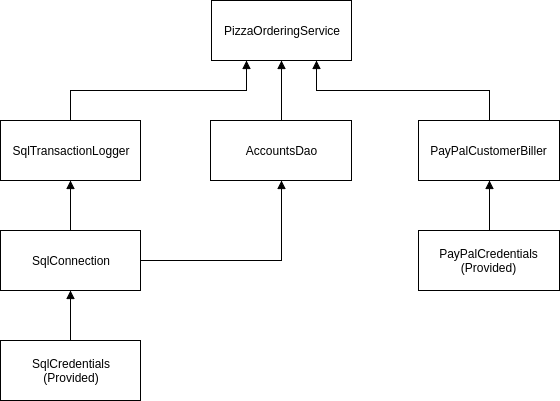
\includegraphics[width=0.7\textwidth]{renders/DependencyInjection.png}
      \caption{Dependency Graph Built by Guice}
      \label{fig:depGraph}
\end{figure}

This leads to extremely simple code for the \java{PizzaOrderingService} in which the logic is entirely separated from the dependency management.

\lstinputlisting[
  caption={Pizza Ordering Service with Dependency Injection},
  label={lst:DI},
  style=javaStyle
  ]{code/technologies/DI.java}

Aside from abstracting away the dependency instantiation, dependency injection also has the added benefit in that all of a class' dependencies become part of the class' constructor signature. There are no required dependencies that are buried within the implementation logic. This makes the code much simpler to test. The \java{PayPalCustomerBiller} used by the class is essentially hardwired into the code that does not use dependency injection (\refcode{lst:noDI}), meaning there is no way to test this class without actually billing a (fake) customer. However as the \java{PayPalCustomerBiller} used by the dependency injected code (\refcode{lst:DI}) is injected into the constructor, a mock of this object (which skips the actual billing, but returns results as if it actually billed a customer) can be passed to the class and used for testing purposes.   

\subsection{Immutables - Immutability for Java}
Immutability is a programming paradigm in which once an object is created, it may never been changed. At first glance this sounds like a bad idea which will result in redundant object creation, but the positives strongly outweigh the negatives. The primary benefit of immutability is that the programmer is \textbf{guaranteed} that any object they hold a reference to, will never be changed. This concept is closely tied to the concept of writing \textit{pure} functions. These are functions which have no external side effects. That is, they take in arguments and return a value, but do not change the input arguments (or any other state contained in the program) in any way. 

These benefits are best highlighted through sample code. Consider the case of a simple website where each login attempt by a user should be logged to a database table in order to detect a hacker trying to crack a password by repeatedly trying to login as the same user. For obvious reasons, this table should not store the user's password (in case of real login attempts), so this should be omitted from the object being logged to the database. An example \java{LoginRequest} is shown in \refcode{lst:loginRequest}. A \java{LoginAttemptLogger} class is written to handle logging these attempts to the database and is shown in \refcode{lst:loginAttemptLogger}. The \java{logLoginAttempt} method handles stripping the password from the \java{LoginRequest} and writing it to the database. 

\lstinputlisting[
  caption={An Example \java{LoginRequest}},
  label={lst:loginRequest},
  style=javaStyle
  ]{code/technologies/immutability/LoginRequest.java}

\lstinputlisting[
  caption={An Example \java{LoginAttemptLogger} Implementation},
  label={lst:loginAttemptLogger},
  style=javaStyle
  ]{code/technologies/immutability/LoginAttemptLogger.java}

However this style of code is a recipe for disaster. The \java{LoginRequest} is \textit{mutable} and the \java{logLoginAttempt} method contains a side effect in that it sets the password of the \java{LoginRequest} to an empty string. Some perfectly reasonable client code is shown in \refcode{lst:clientLoginCode} in which the client logs the login request to the database and subsequently tries to log in. In this case, no user will ever be able to login as all the passwords of the login requests are always mutated to be an empty string. Thus, having \java{LoginRequest} as a mutable object causes a critical bug that will not be caught until runtime. The client login code may check and find that the \java{LoginRequest} contains a password prior to logging the login attempt to the database. However when it goes to finally login, it never will.

\lstinputlisting[
  caption={Perfectly Reasonable Client Login Code},
  label={lst:clientLoginCode},
  style=javaStyle
  ]{code/technologies/immutability/ClientLogin.java}

The solution to this problem is to create a new \java{LoginRequest} without the user's password and log that to the database. This can be done inside of the client login code (defensive copying) before passing the \java{LoginReuqest} to the \java{logLoginAttempt}. However if mutators are provided, it is extremely likely that they will be used somewhere in the code. Thus, the best solution is simply to not provide them at all - make the object entirely immutable. This in turn requires some clunky code inside of the client login method (see \refcode{lst:clunkyImmutableClient}), but avoids the issue caused by the side effect of \java{logLoginAttempt}. 

\lstinputlisting[
  caption={Logically Correct Login Code with Extra Boilerplate},
  label={lst:clunkyImmutableClient},
  style=javaStyle
  ]{code/technologies/immutability/ImmutableClientLogin.java}

The Immutables \cite{immutablesJava} provides a framework for auto generating fully immutable object implementations in Java. These implementations provide extremely useful functionality such as implementing builders and providing methods for updating the fields of an object in an immutable way. The immutable data structure is defined using an interface (annotated with \java{@Value.Immutable}) which contains the \textit{getter} methods for each desired fields of the object. A class which implements this interface in an immutable way is then auto generated by the framework and can is then used in place of the interface. An example of the interface used for \java{LoginRequest} is shown in \refcode{lst:immutableLibLoginRequest}.

\lstinputlisting[
  caption={Interface for \java{LoginRequest} using Immutables Framework},
  label={lst:immutableLibLoginRequest},
  style=javaStyle
  ]{code/technologies/immutability/ImmutableLibLoginRequest.java}

The implementation of this interface generated by the framework then provides a \java{withFieldName} method for each of the fields defined, allowing a new instance of the object with the updated fields to be obtained with a single method call as shown in \refcode{lst:loginAttemptLoggerWithImmutable}. This solves the problem of mutating the \java{LoginRequest} that the client holds a reference to and drastically simplifies working with immutable objects in Java. This framework is used extensively at HubSpot and is a major contributor to the simplicity of writing code without bugs at the company.

\lstinputlisting[
  caption={The \java{LoginAttemptLogger} using the Immutables Framework},
  label={lst:loginAttemptLoggerWithImmutable},
  style=javaStyle
  ]{code/technologies/immutability/LoginAttemptLoggerImmutable.java}


\subsection{Kafka - Streaming Platform}\label{sec:kafka}
Kafka \cite{kafka} is a horizontally scalable, fault tolerant, distributed streaming platform used to read and write streams of data in real time. It is an extremely high performance system and is used extensively by the \team{} team as the primary data pipeline. Kafka runs on its own cluster and stores streams of records inside categories known as Kafka \textit{topics}. Kafka provides two key APIs that are used at HubSpot - one for producing records to a given Kafka topic and one for consuming records from a specific Kafka topic. Kafka is used extensively inside of the team's internal pipeline, but also as an interface between teams. For example, the teams responsible for generating the full HTML body of an email to be sent on behalf of a customer can produce this ready to be sent email to a specific Kafka topic. Kafka consumers owned by the \team{} team are subscribed to this topic and thus pick up these records and can perform the send of the email. This entirely decouples the work done by the two teams. The upstream teams simply put messages onto Kafka to be handled elsewhere. An obvious alternative to using Kafka would be to simply expose a REST endpoint to which the message is POSTed to. However simple HTTP would struggle to support the volume of requests (upwards of 25M emails per day) seen by the \team{} team. As mentioned, Kafka is horizontally scalable, meaning the number of nodes on the Kafka cluster can simply grow as the number of messages published to Kafka increases. Similarly, on the consumer side, the number of deployed consumers subscribed to a given topic can simply be increased in order to meet the increased number of records published to the topic.

Kafka also provides another layer of granularity - partitions. Each Kafka topic is segmented into a number of partitions. Each partition is (at any given time) owned by exactly one Kafka consumer, but each Kafka consumer may own multiple partitions. This leads to an interesting case when choosing the number of partitions to use for a given topic. Ideally, the number of partitions should be a highly composite number \cite {highlyCompositeNumbers}. These are numbers which are divisible by many other numbers, for example 24 which is divisible by 2, 3, 4, 6, 8 and 12. To illustrate why, consider the case where 9 partitions are used - the work load is only equally distributed if 1, 3 or 9 consumers are used. Thus, if 3 consumers isn't enough, scaling to five consumers means four consumers will be consuming from two partitions and one will only be consuming from one partition. Using a highly composite number of partitions allows for more flexibility when choosing the number of consumers, while still balancing the load across the consumers. Kafka can also handle rebalancing the workload, by redistributing the partitions when the number of consumers changes. 

When messages are produced to a Kafka topic, a decision must be made on which partition to assign the message to. This can be done intelligently with load balancing in mind, or simply using a round robin. Partitions can also be replicated in order to provide fault tolerance.

An example of a Kafka topic with two consumers is shown in \reffig{fig:kafka}. 

\begin{figure}[H]
      \centering
      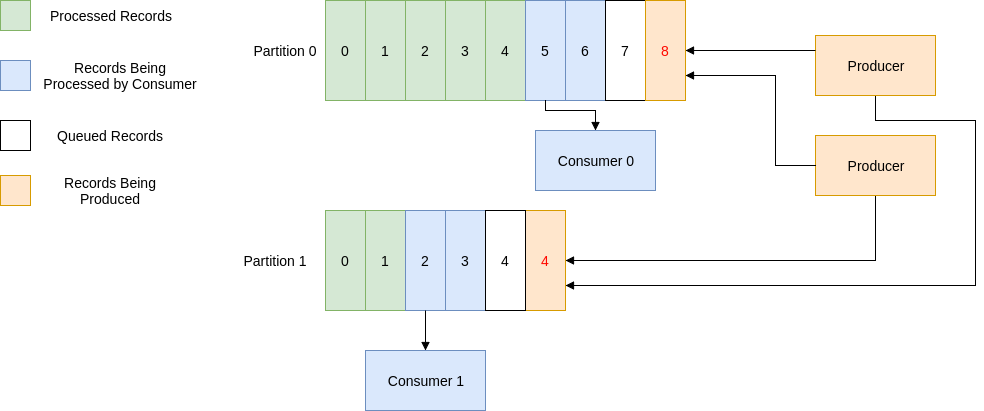
\includegraphics[width=\textwidth]{renders/Kafka.png}
      \caption{Kafka Producers and Consumers}
      \label{fig:kafka}
\end{figure}  

The current situation is outlined as follows:
\begin{itemize}
\item{Consumer 0 has successfully processed (and committed) messages 0 to 4 and is currently processing messages 5 and 6 of partition 0}
\item{Consumer 1 has successfully processed (and committed) messages 0 and 1 and is currently processing messages 2 and 3 of partition 1}
\item{Message 7 in partition 0 and message 4 in partition 1 have both been successfully produced and committed to the log, but not yet processed}
\item{Message 8 in partition 0 and message 4 in partition 1 will be the next messages produced by the producers.}
\end{itemize}

The main purpose of Kafka partitions is to allow records on a single topic to be processed in parallel. As each partition is only owned by a single consumer, the model required for keeping track of what messages have been processed in a certain partition is very simple. However since a consumer may own multiple partitions, the configuration can be tweaked to ensure consumers are always busy. Partitions also aid in keeping records on a single partition isolated. If a bad record appears in a particular partition and the consumer gets stuck trying to process it, only that partition will be impacted.

Each message published to a Kafka partition gets an incremental id known as an \textit{offset}. Consumers are responsible for managing their offset in the message stream. Thus, consumers can be configured to start from any offset, which can even allow for reprocessing of data should the need arise. This has been useful in the past at HubSpot when a bug has caused emails to fail to send. The consumers can have their offsets reset to when the bug first surfaced and the emails will be resent. However this is a delicate process and is only used as a last resort. The offsets for consumers 0 and 1 in \reffig{fig:kafka} would be 4 and 1 respectively.

A key concept to understand about Kafka is that consumers are presented with batches of records, of a configurable size. The batch size in \reffig{fig:kafka} is two. The records inside the batch may be processed out of order, but the batch of records is considered completed \textbf{only when every record in the batch has been processed}. In Kafka, only an entire batch of messages can be marked as processed. For example consider consumer 1 in \reffig{fig:kafka}. Should the consumer succeed to process message two, but fail to process message three, Kafka must be notified of the failure to process the batch of messages (or will notice a timeout) and the entire batch will be retried.


Another interesting concept in Kafka is consumer groups. Consider the case where two entirely separate sets of consumers (running different code) need to read from the same Kafka topic. Both sets of consumers should be able to process every message that is published to the topic and this is what consumer groups provides. Without consumer groups, another consumer could be set up in order to read from the Kafka topic, but as discussed, it would only acquire a certain number of partitions and thus miss some messages (and steal messages from existing consumers). The solution is to specify the consumer group that each running consumer belongs to. In this case, since there are two sets of consumers, both doing different things, there should be two consumer groups. Kafka will then treat all the consumers in each consumer group as if there are no other sets of consumers reading from the Kafka topic. This feature is best understood by considering the two edge cases:

\begin{itemize}
\item{If all consumers are in the \textit{same} consumer group, Kafka simply load balances the partitions across the number of consumers}. Each consumer will see a \textit{subset} of the records published to the Kafka topic, depending on the partitions owned.
\item{If all consumers are in \textit{different} consumer groups, each consumer will have its own offset in \textbf{all} of the partitions. That is, the consumer responsible for partition zero in consumer group A may have a current offset of 100, while the consumer responsible for partition zero in consumer group B may have a current offset of 0. This is essentially, publish-subscribe (pub-sub) behavior. All the consumers will simply see all the records and the rate of consumption of a certain consumer has no impact on the rate of consumption of another consumer.}
\end{itemize}

Continuing with the previous example of having all the emails to be sent through HubSpot contained on a Kafka topic, the following consumer groups could be set up in order to both send every email that appears on the topic and to bill the customer for each email they send. This is shown in \reffig{fig:consumerGroups}
\begin{labeling}{Sending CG}
\item[Sending CG]{This consumer group would contain all the \team{} team's consumers. There would likely be a lot of consumers in this consumer group in order to keep up with the time consuming process of actually sending the emails on behalf of the customers. These consumers would need to be as efficient as possible and the delta between the current offset (the index of the most recently produced message) and the oldest offset (the index of the oldest message still being processed) for each partition would likely be carefully monitored to ensure the consumers are not falling behind}
\item[Billing CG]{This consumer group would perhaps simply read the account number of the customer sending the email and bill that customer. This consumer group would be considerably less time critical and would likely only need to perform some light weight task for each message on the Kafka topic.}
\end{labeling}


\begin{figure}[H]
      \centering
      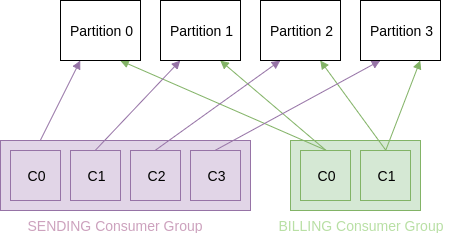
\includegraphics[width=0.6\textwidth]{renders/ConsumerGroups.png}
      \caption{Partition Assignments with Multiple Consumer Groups}
      \label{fig:consumerGroups}
\end{figure}  

A final note of interest regarding Kafka is that it provides an \textit{at-least-once} guarantee that messages will arrive at consumers for processing. If a single message in a batch of messages cannot be processed for whatever reason, the entire batch will be retried. Thus, external idempotency logic is required in order to obtain an \textit{exactly-once} processing guarantee. The \team{} team uses a simple HBase table in order to lock each email that is to be sent, prior to actually sending it. 

\subsection{Hadoop - Big Data Processing}\label{sec:hadoop}
 As with most modern companies, HubSpot's platform generates a monumental amount of data. This data can be leveraged to gain extremely useful insights into how the platform is used, how certain systems are performing and what should be targeted by engineers working on the product. As discussed in \refsec{sec:kafka}, Kafka is used throughout HubSpot to provide high performance data streams. This is ideal for things like moving an email through the entire pipeline from design to sending. However, the contents of Kafka topics are often also persisted (for example for 30 days) to Amazon Web Service's cloud storage facility, Amazon S3 \cite{s3} . Persisted Kafka topics provide a huge amount of data which is typically critical to a system's operations if Kafka is used in the first place. 
 
 Hadoop is a framework that allows for the distributed processing of large data sets across clusters of computers using simple programming models \cite{hadoop}. Often times the size of the datasets persisted to S3 would be too large to hold on disk of a typical machine, and certainly not in memory. Hadoop is horizontally scalable allowing for more and more machines to be added to a cluster as demand grows. Hadoop is used extensively at HubSpot for processing these huge volumes of data by writing Hadoop jobs. These are jobs which make use of the Hadoop framework and run on a cluster created specifically for Hadoop jobs. These jobs can be scheduled and used to periodically hydrate some other data store, or on demand and used when a certain question needs to be answered. 
 
 An example of a scheduled job used by the \team{} team is one which aggregates all the sending statistics for a given HubSpot email sending account. This is used to hydrate an SQL table, which backs an internal dashboard which is used to gain insights into the system. Large customers can potentially send hundreds of thousands, or occasionally millions, of emails in a given day. As discussed, all these emails are contained in Kafka and persisted to S3. In order to extract the useful information, these files need to be indexed and aggregated. Several key values can then be derived from this data such as the percentage of emails sent from this account that were delivered first time, the breakdown of the reasons emails sent from this account were rejected (e.g. the IP has a bad reputation) and many others.

Hadoop offers a large number of benefits. Hadoop is fault tolerant - for example if a mapper node dies and produces no output, the corresponding map process will be repeated on another node. Hadoop make use of the \textit{Hadoop Distributed File System (HDFS)} \cite{HDFS} which provides data replication and support for huge datasets. One of the key benefits of using HDFS that Hadoop leverages is that it can attempt to assign work to nodes based on the data they \textbf{already have}. This limits the costly operation of moving data around the network. This is succinctly summarized by Hadoop's famous design ethos - \textit{"bring the processing to the data"}.

The main user facing API contained in Hadoop, is Hadoop Map-Reduce. Map-reduce is a programming model for highly parallelizable data processing. The map-reduce methodology consists of four key phases - \textit{split, map, shuffle, reduce}. As an example, consider a dataset which is a corpus of quotes of the form:
\textit{"Learning never exhausts the mind - Leonardo da Vinci"}. An example task on this dataset would be to calculate the number of quotes contained by each of the authors in the corpus. This would be implemented using map-reduce in the following manner:

\begin{labeling}{Reduce }
	\item [Split] The initial step would be to split the corpus into chunks for processing on different nodes in the cluster. As discussed, Hadoop does this intelligently by trying to assign chunks for processing to worker nodes who already contain that data. This phase would output a single record for each quote in the corpus.
  \item [Map] This is the beginning of the useful processing of the data. The purpose of the map phase is to output a key-value pair. In this example, the key would be the name of the author and the value would simply be one, as each entry in the corpus is a single quote. The map phase would likely require a regular expression to parse the name of the author from the quote.
  \item [Shuffle] The \textit{shuffle} phase is responsible for grouping the output key value pairs produced by the map phase by key. This forms a list of the values that are associated with each key from the map phase. In this example, a possible output of the shuffle phase would be: \java{Leonardo da Vinci -> [1, 1, 1]}, indicating that three entries with the key ``Leonardo da Vinci'' were found and each had a corresponding value of 1. 
  \item [Reduce] The final phase is the \textit{reduce} phase. The input to the reduce phase is the output of the shuffle phase - a key and a collection of values associated with that key. As the name suggests, the reduce phase is responsible for reducing this collection of values down to a single value. In this example, the single value output of the reduce phase would simply be the number of elements in the collection of values, indicating the number of quotes found by the particular author.
\end{labeling}


\subsection{Protobuf - Structured Data Serialization}\label{sec:protobuf}
Protocol Buffers (Protobuf) are Google's language-neutral, platform-neutral, extensible mechanism for serializing structured data \cite{protobuf}. Protobuf is similar in concept to XML or JSON, but produces data which is 3 to 10 times smaller in serialized form \cite{protobufSizeStat}. Protobuf also offers many powerful features such as enums, types, default values and nested messages.

Protobuf works by defining the desired data structures in a special .proto file. Compilers exist for a large number of languages (e.g. Java, C++, Python etc) which compile these .proto files into classes usable inside the language. For example the Java Protobuf compiler generates immutable Java objects with a variety of useful features such as builders and methods for serializing and deserializing to and from immutable byte arrays. The serialization / deserialization process is extremely fast and is especially useful in conjunction with Kafka (see \refsec{sec:kafka}), which operates solely on byte arrays. An example of a Protobuf message for a person is shown in \refcode{lst:protoPerson}. This example shows the rich features such as optional fields (email), enums (PhoneType), nested messages (PhoneNumber) and arrays of values (PhoneNumber).

\lstinputlisting[
  caption={A Protobuf Representation of a Person},
  label={lst:protoPerson},
  style=protoStyle,
  ]{code/technologies/person.proto}

\subsection{gRPC - Remote Procedure Calling}
gRPC is a cross language remote procedure calling framework \cite{gRPC}. It serves as an alternative to the current de facto standard of having services communicate using REST endpoints over HTTP/1.1. gRPC operates by defining a service and specifying the methods that can be called remotely, along with their parameters and return types \cite{gRPCDef}. gRPC uses Protobuf (see \refsec{sec:protobuf}) as its IDL (interface definition language). That is, the defined methods (by default) accept as parameters, and return, Protobuf messages. As with Protobuf, compilers exist for a variety of languages which generate the client side and server side code for their respective languages. Clients of the service can then remotely invoke these methods on objects they hold known as \textit{stubs}. The methods are then remotely invoked on the server. To the client, the procedure call appears no different to any other procedure call as all the remote networking is handled by the framework. 

gRPC is built upon HTTP/2 which offers many new powerful features. One of the main advantages of HTTP/2 over HTTP/1.1 is multiplexing which allows multiple HTTP requests to be made (and responses received) asynchronously over a single TCP connection. The enables the gRPC framework to provide four types of RPC invocations:

\begin{enumerate}
  \item{The first type of call is a simple \textit{unary} call. In this case, the client sends a single request to the server, who handles the request and returns a single response. This is equivalent to a typical HTTP/1.1 request and response.}
  \item{The second type of call is \textit{server side streaming}. In this case, the client sends a single request to the server and the server responds with a stream of messages. This is useful in cases where the response may be a large collection of items. The client may not need \textbf{all} of the items before it can begin processing. Thus, the server can respond with a stream, allowing the client to begin reading messages from the stream as they become available.}
  \item{The third type of call is \textit{client side streaming}. This is the exact opposite to server side streaming and is useful in cases where the client must send a lot of data, but the server can begin processing that data before it has all been received.}
  \item{The final type of call is \textit{bidirectional streaming}. As expected, this is when both the client and server communicate using streams. These streams are entirely independent from one and other, allowing the client / server to read messages in any order.}
\end{enumerate}

The \team{} team uses gRPC at the final stage of the email sending pipeline. The last step is to get the email to the servers which are responsible for sending the email to the recipient using SMTP (see \refsec{sec:smtp}). As discussed in \refsec{sec:emailSendingInfra}, SMTP email sends can take on the order of seconds. This leads to a very asynchronous system which causes issues if using standard REST endpoints over HTTP/1.1. 

gRPC is used in this case instead of Kafka as particular emails \textbf{must} be sent from particular IP addresses for SPF to pass (see \refsec{sec:DNS} for more information on SPF). Certain email sending servers will be bound to certain public IP addresses, meaning certain emails \textbf{must} be sent from certain servers. If Kafka was used for the final step, there is no guarantee that the consumer who owns the partition the email ends up in will be bound to the correct IP address, meaning they would not be able to send the email. gRPC can be used to connect to the server who is \textbf{known} to be bound to the correct IP address. This could also accomplished using a simple REST endpoint, but as discussed, this causes performance issues.

\section{Email Specific Technologies}
\subsection{Domain Name System (DNS)} \label{sec:DNS}

Although not entirely email specific, DNS is extremely critical for the \team{} team. Aside from teams working on the HubSpot development platform (that is teams working on the platform which engineers develop HubSpot products on), most other teams need not concern themselves with DNS at all. However as DNS is such an important component of email, DNS records must be carefully maintained. For email, there are five key DNS record types, outlined below.

\begin{labeling}{DKIM }
  \item[A] A records are used extensively in DNS. These records define the IP address that is associated with a particular domain. For example, the IP address of the web server which hosts the website \textit{hubspot.com} can be obtained by performing a DNS lookup for the A record associated with \textit{hubspot.com}. This address translation is done every time a user visits a website and enables the use of memorable, human friendly domain names instead of raw IP addresses.
  \item[MX] MX (Mail Exchanger) records are similar to A records except they define the \textbf{hosts} which can accept mail for a given domain. For example, if an email is to be sent to \textit{billing@hubspot.com}, the email sender must know where to send that email. Thus, an MX lookup is performed for \textit{hubspot.com}, the domain in which the account associated with the email address \textit{billing@hubspot.com} resides on. This typically returns a host name, for example, \textit{mx.hubspot.com}. Thus, a subsequent A record lookup for \textit{mx.hubspot.com} is required to determine the exact IP address(es) of the server(s) which can accept email for \textit{billing@hubspot.com}.
  \item[SPF] SPF (Sender Policy Framework) records are used to authorize a set of IP addresses which a domain intends to send email from. The friendly-from address of an email (the sender's address) is simply a plain text header contained in the email. This means that anyone could potentially send email as someone else by spoofing the friendly-from address. SPF records provide part of the mechanism which solves this problem. A domain can declare a list of IP addresses it intends to send email from using an SPF record. Thus, when an email is received from \textit{stefano@example.com}, the SPF record associated with \textit{example.com} can then be fetched and if the source IP address of the email does not match one of the declared IP addresses, the email may be blindly accepted, tentatively accepted or dropped entirely. An example SPF record would be \java{v=spf1 ip4:1.2.3.4/30 -all}. The first component (\java{v=spf1}) indicates the SPF version in use, the second component (\java{ip4:1.2.3.4/30}) is a CIDR representation of the IP addresses this domain authorizes (see \refsec{sec:CIDR}) and the final component (\java{-all}) indicates that email sent from all other IP addresses except the ones defined here should be dropped. 
  \item[PTR] PTR records are the inverse of A records and are used to determine the host associated with a particular IP address. 
  \item[DKIM] DKIM (DomainKeys Identified Mail) records provide another level of authentication. DKIM uses asymmetric-key cryptography to digitally sign emails, verifying that the email was sent by an authorized sender (provided only authorized senders hold the private key). The public component of DKIM keys are contained under the \java{_domainkey} sub domain and are prepended with a DKIM \textit{selector} indicating which DKIM key was used. The \textit{DKIM-Signature} header is included in the email, an example of which is shown in \refcode{lst:dkimSig}.
  \lstinputlisting[
  caption={An Example DKIM signature},
  label={lst:dkimSig},
  style=protoStyle,
  ]{code/technologies/dkim.txt}

  The most important DKIM tag-value pairs are outlined below \cite{dkimSig}:
  \begin{labeling}{bh }
    \item[v] This indicates the DKIM version in use
    \item[a] This indicates the algorithm used to generate the signature.
    \item[s] This is the selector prefix and is used to pick the public key to use from those available at the \java{_domainkey} subdomain.
    \item[h] This contains the list of headers which were hashed to generate the \textit{b} tag
    \item[b] This contains the Base-64 encoded hash of the headers listed in \textit{h}
    \item[bh] This contains the hash of the body of the email
    \item[d] This contains the domain in which the corresponding public key can be found
  \end{labeling}

  The corresponding public key can be found by performing a TXT lookup of \java{<s>._domainkey.<d>}, or in the above case \java{dk1._domainkey.example.com}. The value of these records also contain tag-value pairs, such as \textit{k} which indicates the cryptography system used and \textit{p} which contains the public key itself. Once the public key has been obtained, the inverse of the signing operation can be applied to ensure the email came from an authorized sender.
\end{labeling}


\subsection{Simple Mail Transfer Protocol (SMTP)} \label{sec:smtp}
SMTP is the protocol used for sending email to a mail server. SMTP is quite an old protocol, with the first RFC being published in 1982 \cite{smtpRfc}. For an email to be sent from one machine to another, a connection must be opened up between the mail server responsible for the sender's email and the mail server responsible for the recipient's email. SMTP defines the way in which messages should be exchanged between these two servers. Most mail servers today support 
Extended SMTP (ESMTP), which is outlined in RFC 1869 \cite{esmtpRfc}. This defines a format for indicating which extensions a given SMTP server supports. 

SMTP contains 6 main steps to send email:
\begin{labeling}{MAIL FROM: }
  \item[EHLO] The first SMTP command of interest is \java{EHLO <SMTP domain>}. This is the first message expected by the server. In turn, the SMTP server will respond with a 250 OK message and list all the extensions it supports. 
  \item[MAIL FROM:] The sender then specifies the mail from address to be used for the email (who the email was sent from) using \java{MAIL FROM: <from_email_address>}. Again, provided the server accepts the email address as valid, the server should return a 250 OK.
  \item[RCPT TO:] The sender then specifies the email address that the SMTP server should deliver the email to using \java{RCPT TO: <recipient_email_address>}. Provided the SMTP server accepts responsibility for this recipient address (it expects to receive email for this address), the server will again respond with a 250 OK. Otherwise, the server will reject the message and terminate the connection.
  \item[DATA] The sender then indicates that it wishes to begin sending the data contained in the email message, by sending the \java{DATA} command. The server will then return with a 354, along with some instruction on how to terminate the message, indicating that the client may begin to send the message.
  \item[<content>] The sender then proceeds to send the content of the email message line by line, followed finally by a specific message indicating that the content is completed. This termination message is a single period character on its own line. The server should again respond with a 250 OK once the content has been received.
  \item[QUIT] Finally, the sender issues a \java{QUIT} command. The server will respond with a 221 message and the session may be safely terminated.
\end{labeling}

As the name suggests, SMTP is quite a simple protocol. Many libraries exist which handle SMTP messaging exchanges. However as this needs to happen for every single email that is sent through HubSpot, the \team{} team implemented their own Java high performance and open source SMTP library, NioSmtpClient \cite{hubspotSmtp}. This SMTP client supports several of the SMTP extensions such as TLS which provides encryption and SMTPUTF 8 which supports sending UTF8 characters over SMTP. It also allows connections to be recycled and can automatically determine most efficient sending method based on the EHLO response from the server.     

\section{System Management and Health Monitoring}
While working on projects of this magnitude, bugs and issues are an inevitability. The amount of traffic seen by these systems compounds any small issues or bugs present in the system. As such, it is critical to have systems in place which monitor the health of the system and inform the team of any potential issues with the system. What's more, these issues must be continuously examined and remedial action must be taken where applicable. The \team{} team makes use of several tools and methods for monitoring the health of their systems, a subset of which are outlined in the following sections.

\subsection{Log4j2}\label{sec:log4j2}
Log4j2 \cite{log4j2} is a Java framework which is provides facilities for logging to different log levels and advanced log filtering (for example with regular expressions). This provides an excellent facility for understanding why systems are behaving unexpectedly in production. A common pattern is to insert log messages to a low priority log level (e.g. DEBUG) which describe the state of the system or the code path taken. Typically, when the system is behaving normally, a higher priority log level is set (e.g. INFO) meaning these finer grained log messages are skipped. However, should an issue arise, the log level can then be easily switched to the lower priority temporarily to get a more detailed insight into why the system is misbehaving. This pattern allows detailed log messages to be produced only when they are needed, reducing the amount of noise present in the logs. The framework also provides the ERROR level which can log error messages as uncaught exceptions without killing the currently executing thread.

\subsection{Sentry}
Sentry \cite{sentry} is an online platform which logs uncaught exceptions that arise during program execution. This greatly simplifies the task of finding out the reason for a system fault or failure without the need to trawl through pages of log files. Sentry logs the full stack trace associated with an exception, the time of occurrence and other pieces of metadata such as the name of the deployable. It uses this data to monitor the occurrences of particular exceptions over time, provides facilities for opening and closing GitHub issues and most importantly, to send an email to all those subscribed to the project (e.g. the \team{} team in this case) when an exception occurs. Sentry proves to be extremely useful at deploy time. Obviously when deploying new code to production servers, one must be sure that the changes did not cause the system to enter an unhealthy state. Provided the code is well written and that unexpected exceptions that occur are not silently swallowed, Sentry can be monitored at deploy time in order to help provide the engineer with confidence that the deployed changes were non breaking. Sentry also provides support for integrating into Log4j2 (see \refsec{sec:log4j2}). Sentry can monitor ERROR level log messages that are produced by Log4j2 and subsequently log these error messages to the Sentry platform. As an engineer this combination of tools is extremely useful for indicating that the system has found an issue, without killing the thread. This is ideal in cases where some work has been done and the system has encountered a critical error, but does not need to be restarted. This mitigates the need to repeat the work, but still informs the team that an error has occurred by logging an exception to Sentry.

\subsection{SignalFX}
SignalFX \cite{sigfx} is an online tool for recording metrics and data visualization. Gathering and analysing metrics is a key part of ensuring the health of a complex system. When things start to fail, SignalFX is the first place engineers look to. SignalFX essentially allows data to be dumped to the cloud and for complex graphs and charts to be rendered in real time using this data. SignalFX supports creating dashboards consisting of many of these graphs and charts. The \team{} team has several of these dashboards, each encapsulating a single part of the system. When problems inevitably arise, the team can examine these dashboards in order to try to isolate and find the problem. Once remedial action has been taken, the dashboards can be monitored to ensure the desired effect takes place. Being able to see these metrics in close to real time is incredibly useful for diagnosing faults with the system. It also serves as an excellent mechanism for finding parts of the system that can be improved. For example, critical code paths can be timed and the results logged to SignalFX. This allows accurate inferences to be made about parts of the system and allows the team to target parts of the system which need improvement.

SignalFX also allows for detectors to be configured. For example, a chart could be created monitoring the number of emails sent in the past minute by each IP address responsible for sending emails. A detector can then be put in place to detect if this number falls below a certain threshold. Detectors can be configured to alert via email and Slack when they trigger, allowing engineers to be notified. 

SignalFX also supports complex data aggregations. This is beneficial as it decouples calculations that need to be done on metrics from the code which the metrics are monitoring. Performing any sort of data manipulation in performance critical code paths is obviously not desirable when every millisecond counts. Instead, metrics gathering is as simple as producing the data to SignalFX. The complex graphs and charts can then be configured inside of the SignalFX tool, entirely independent to the production code. 
\chapter{Tasks Undertaken}
Throughout the course of the internship, a variety of tasks were undertaken and completed.  
For the sake of brevity a small subset of the most interesting of these tasks are outlined below. 

\section{Rebuilt DNS Management System}
DNS plays an important part in sending emails. As discussed in \refsec{sec:DNS}, there a several DNS records that must be maintained for a server to send email. As HubSpot aims to offer as seemless an experience as possible to its customers, it attempts to take care of as much of the DNS settings as possible on behalf of the customer. Ultimately however, if a customer want's HubSpot to send their marketing emails through an SMTP domain of \java{emails.company.com}, these DNS records must be obtainable at that domain as discussed in \refsec{sec:DNS}. 

As things change at HubSpot, it is quite likely that these DNS records would need to change over time. For example, if the customer should add another dedicated IP address to their account, this would have to be added to their SPF record. At first glance this would require HubSpot's customers to be frequently changing their DNS records, something most customers would not be overly comfortable with. The solution to this problem, as with so many problems in computer science, is indirection. 

The Domain Name System supports the concept of including other DNS records, even from entirely different domains. This is exactly the behavior that lets HubSpot manage their customers' DNS on their behalf. For example, instead of \java{emails.company.com} having the SPF record which contains their allowed sending IPs and having to change it should their sending IPs change, they can simply setup this record as a pointer to another DNS record, a record on HubSpot's domain. Clients who require the SPF record for \java{emails.company.com} will be informed to use the record contained on HubSpot's domain instead. An example of this is shown in \reffig{fig:dnsIncludes}, where 99 is the customer's HubSpot identification number. A similar setup exists for customers' DKIM records.

Thus, the customer only ever needs to set up the DNS pointers to HubSpot's domain once. Once that is done, HubSpot can control the actual values of those DNS records on behalf of the customer. 

\begin{figure}[H]
      \centering
      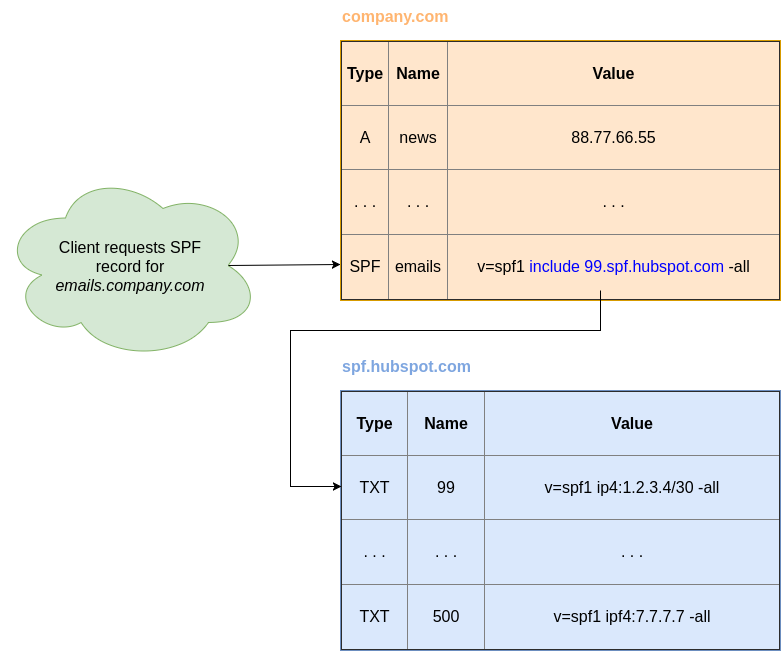
\includegraphics[width=0.8\textwidth]{renders/DnsIncludes.png}
      \caption{DNS Includes for \textit{emails.company.com}, HubSpot Customer 99.}
      \label{fig:dnsIncludes}
\end{figure}

Initially, all the DNS records that the customers include were created at various points in the code. There was no definition for exactly what DNS records should be available and where they should be available for a given account. Some of the DNS record creation was coupled to the code that was responsible for creating new customer accounts, but as time went on, different DNS records were required, resulting in redundant DNS records being created. There were also several cron jobs (jobs which run on a schedule) responsible for checking the current status of the DNS records and attempting to adjust them as necessary. There was also no unit tests for any of the code which synced DNS records. Some of these jobs concluded that different values should exist for the same DNS record, resulting in the jobs competing with each other and updating DNS records every time they ran. It was also unclear what DNS changes were required if accounts were updated. This led to the creation of an entirely new DNS management system.


\subsection{Requirements for the Management System}
Prior to beginning to rebuild the system, an analysis of the current system was required to ensure all the required functionality contained in the old system would be included in the new system. Another important step was to consider what the \textit{ideal} system would look like. There were two main options to consider:

\begin{enumerate}
    \item{Create all the DNS records required when the corresponding customer account was created. As discussed previously, it is likely that the value of these DNS records would change over time. Thus, this would also require periodic cron jobs in order to compare the current state of a customer's DNS records against what the system believes their DNS records should be and to update them accordingly. The downside to this approach was having the required DNS records defined and maintained in two separate places - once during account creation and once during the DNS record synchronization.}
    \item{Abstract away all DNS record creation from the account creation process and write the periodic cron jobs in such a way that they can also create brand new DNS records as necessary. The downside of this approach is that there would be a period of time in which the accounts would be created, but have invalid DNS records, which could be problematic if not managed appropriately.}  
\end{enumerate}

After some consideration, it became clear that option two was the better choice. The period of time in which the accounts would be created but have invalid DNS records could be managed rather simply. Provided the jobs were written correctly, this approach would have the benefit that it could sync DNS records for arbitrarily complex entities. For example, initially the customer's account was all that was required in order to keep their DNS records in sync. However as time went on, other types of DNS records also needed to be maintained, which could not necessarily be deterministically generated from just a customer's account. An example of this is IP addresses which are owned by HubSpot, but not yet in use by any customer. These IP addresses should have specific DNS records in place. However by definition, these IP addresses are not yet assigned to any accounts. Thus, the new system should also be able to sync DNS records based on IP addresses. In the past the solution to this problem would have been to simply create yet another periodic cron job to maintain those DNS records, making it even more difficult for an engineer to know where in the code a given DNS record is maintained.

Another important concept are DNS \textit{zones} (sub domains). For easier organization and management of a large number of DNS records, a top-level-domain (TLD) can be further sub-categorized into zones. In the previous example domain \java{emails.company.com}, the TLD is \java{company.com} and a zone on that TLD could be created for \java{emails}. The purpose of DNS zones is to allow finer grained control for a domain with a large number of DNS records. For example, a customer could setup all the records required for HubSpot's email marketing on a single zone, the \java{emails} zone, isolated from all the domain's other records (e.g. for their website, internal email etc). 

The requirements of the new system were determined to be the following:
\begin{enumerate}
      \item{It can sync DNS records for arbitrary entities (Accounts, IP Addresses etc)}
      \item{The code for generating the values of specific DNS records should be decoupled from the code which actually runs the job. This allows for comprehensive unit testing of the code which generates the records.}
      \item{It should only make external requests to update records which are no longer valid.}
      \item{It should group the records required for a given entity by zone, allowing for easier record lookups and updates}
\end{enumerate}

\subsection{Implementation of the System}
The first task was to decide how the code which builds the DNS records should be organized. It was imperative to have this code be as clear and concise as possible. The DNS records themselves are hosted on various providers (e.g. Cloudfare), but the Platform team in HubSpot provides a simple client for working with these records (creating records etc). A \java{DnsRecordBuilder<T>} interface was defined and is shown in \refapp{appendix:dnsManagement} \refcode{lst:dnsRecordBuilder}. This interface defines the following methods:

\begin{itemize}

      \item{\java{Multimap<String, RecordRequest> buildSpfRecords(T entity)}}
      \begin{itemize}
            \item{This method will generate the SPF records required for a given entity of type \java{T} (e.g. an account)}
            \item{Equivalent methods are also defined for MX, A and DKIM records}
            \item{The \java{RecordRequest} object is a Java object whose contents can be passed to the DnsClient library to create / update / delete the given record}
            \item{These methods return Multimaps (which is essentially a \java{Map<String, Collection<RecordRequest>>}) which use the record's zone as the key}
            \item{All these methods are defaulted to returning empty multimaps (if they are not overridden)}
      \end{itemize}

      \item{\java{boolean appliesTo(T entity)}}
      \begin{itemize}
            \item{This method specifies whether or not this particular implementation of \java{DnsRecordBuilder} should apply to this entity}
            \item{For example if the entity was an account, this method can be used to specify that only accounts with dedicated IP addresses should use this \java{DnsRecordBuilder}}
      \end{itemize}

      \item{\java{Map<String,DnsConfiguration> getDnsConfigByZone(T entity)}}
      \begin{itemize}
            \item{The \java{DnsConfiguration} is a Java object which contains a zone name and a list of \java{RecordRequest} objects (which contains all the records to be created)}
            \item{This method has a useful default implementation which aggregates all the multimaps returned by each methods that builds the records of each type (SPF, DKIM, A, MX) into a single multimap. The returned map of DNS configurations by zone can then be built and returned.}
            \item{This is the most common method called on this interface as it invokes all the other methods, returning the exact DNS configurations (by zone) needed to keep the given entity up to date.}
      \end{itemize}

      \item{\java{Map<String, String> buildPtrRecords(T entity)}}
      \begin{itemize}
            \item{The final method defines the PTR records that should be created for this entity, returning a map containing the IP address as the key and the host name corresponding to this IP address as the value}
            \item{As discussed in \refsec{sec:DNS}, PTR records are used to perform reverse A lookups, defining the host name associated with an IP address.}
      \end{itemize}
\end{itemize}

Implementations of this interface can then be created for a given entity type. For example, a \java{DefaultAccountDnsRecordBuilder<Account>} was created to encapsulate all the records that need to be created for every HubSpot customer account. Similarly, a \java{UnassignedIpDnsRecordBuilder<IpAddress>} was also created to encapsulate all the DNS records required for an unassigned IP address. The \java{IpAddress} object contains the status of the IP address (whether its associated with a customer account or not). The \java{appliesTo} method of this implementation can then check this field and only return DNS records if the \java{IpAddress} is in fact unassigned. As time went on, more of these \java{DnsRecordBuilder} implementations were created, encapsulating different DNS requirements. This provides a very clean and extensible way of defining DNS records which are deterministically built from arbitrary entities.

The next step in the implementation was to write an intermediate class which given an entity of type \java{T}, applies all the \java{DnsRecordBuilder}s corresponding to the entity and finds out which records need updating. 

A \java{Map<Class, List<DnsRecordBuilder>>} is created and is used to determine the list of \java{DnsRecordBuilder}s that need to be applied to a given entity by simply looking up the entity's class in the map. The \java{getDnsConfigurationsByZone} method defined above is invoked on each of the builders in the list, generating all the DNS records that need to be present for the given entity. 

Finally, another piece of logic was written to determine which records need to be updated for the entity. This is done by checking the records against an in-memory cache, a database cache and finally live DNS. This reduces the number of real DNS queries that need to be made. The in-memory cache and database cache would be frequently invalidated to ensure cached DNS records had not become stale. Any records which require updates are then added to a \java{List<DnsConfiguration>} and returned to the caller to perform the actual updating. This code segment is provided in \refapp{appendix:dnsManagement} \refcode{lst:recordBuilderApplier}.

The final step was to create the cron job which will use the above code to keep the required DNS records in sync. The HubSpot development platform provides a simple means of registering jobs which are to be run on a schedule. The benefits of the extra complexity of the above code are seen in the implementation of the job. The job simply fetches all the entities of interest (\java{Account}s, \java{IpAddress}es etc) from a database. For each of these entities, the job calls the method from the intermediate class as discussed in the previous paragraph using the entity as a parameter. This method returns the list of records which need be updated or created. The job then handles performing the required DNS updates. A simplified version of the job in which the DNS records for all accounts are synced is shown in \refapp{appendix:dnsManagement} \refcode{lst:dnsSyncJob}.

\break
\section{CIDR Minimization Algorithm}
As discussed in \refsec{sec:DNS}, SPF records are a vital part of authorization when it comes to sending emails. SPF records are typically used to specify a set of IP addresses that a particular domain may send emails from. An important aspect of SPF records (or more specifically, the underlying TXT record) is that the length of the entire record value (which is a simple string) should be at most 255 characters as per RFC 7208 \cite{spfRFC}. Given the fact that a particular HubSpot customer may potentially send email over any one of tens of HubSpot owned IPs, this can cause problems. 

One of the upgrades customers can avail of is purchasing dedicated IP addresses, which will be used for their email traffic and theirs only. This allows the customer to build up a good IP reputation without the risk of the reputation being harmed by other HubSpot customers who may send lower quality email. HubSpot owns a large number of IP addresses in order to facilitate this. One of the other tasks undertaken during the internship was automating the process of setting up email sending accounts for new dedicated customers. Prior to this automation, one of the decisions that needed to be made by support staff working with customers was which IP address(es) to assign to customers. Some customers have existing IP addresses and IPs should be selected in order to minimize the length of the resulting SPF record that the customer will have. SPF records support CIDR notation (see \refsec{sec:CIDR}) of IP addresses, meaning smart IP selection can save valuable characters in a customer's SPF record. Thus, an important step in automating the setting up of customer accounts with dedicated IP addresses was automating the IP address selection, while still minimizing the resulting SPF records.

\subsection{CIDR Notation} \label{sec:CIDR}
CIDR (Classless Inter-Domain Routing) notation is a compact way to represent an IP address along with its associated subnet mask and network prefix \cite{cidr}. With regards to SPF records, it is useful as it can be used to compactly represent a set of IP addresses. This set consists of the IP addresses of all the hosts on the sub-network (subnet) specified by the network prefix. This section will primarily discuss CIDR notation for version four (IPv4) IP addresses, though all the same logic holds for version six (IPv6) IP addresses. 

Typically, IP addresses are represented as quartet of period separated integers ranging from 0 to 255, for example, $192.168.1.1$. However, this representation is simply employed in order to make reading IP addresses easier for humans. In actuality, version four IP addresses are more simply represented as 32 bit integers. Each of the numbers in the quartet can take on one of 256 values. Thus:

\begin{equation}
\begin{split}
\log_2 256 = 8\,bits\,per\,element\,in\,quartet \\
8\,bits\,per\,element \times 4\,elements\,in\,quartet = 32\, bits
\end{split}
\end{equation}



$192.168.1.1$ could be represented as a 32 bit integer by using $192$ as the upper (most significant) 8 bits, $168$ as the next 8 bits and so on. CIDR notation contains the IP address in question, followed by a slash and a number, for example $192.168.1.2/31$. CIDR notation partitions the 32 bit representation of the IP address into two pieces - the upper bits make up the network prefix and the remaining bits are used to specify the specific host on that network. The number following the slash denotes the number of bits to use for the network prefix. Thus, $192.168.1.3/31$ specifies that 31 out of the 32 bits should be used for the network prefix and all other bits should be zeroed in order to obtain the network address. This implies that the network address is $192.168.1.2$. This is because the least significant byte of this IP address is 3, or $(0000\enspace0011)_2$ in binary, and the last bit is to be zeroed meaning the last byte of the network address becomes $(0000\enspace0010)_2$, which is 2 in base-10. 

CIDR notation can thus be used to represent a set of IP addresses, provided they are contiguous. The set has a cardinality that is an integral power of 2 and the first IP address in the set lies on a CIDR boundary. The set of IPs $\{192.168.1.0,\enspace192.168.1.1\}$ can be represented using CIDR notation as $192.168.1.0/31$. The logic here is that the address of the subnet containing the hosts of interest is provided and the implied set of IPs is the set of all IP addresses of the hosts on that subnet.  Thus, if a customer owns these two IP addresses, their SPF record can simply contain the CIDR notation value of the subnet which contains the two IP addresses, reducing the number of characters required by almost half. This is due to the fact that $/31$ implies that there is one bit (the last bit) which identifies the host on the subnetwork defined by $192.168.1.0$. This bit can either be a zero or a one, yielding the two possible IP addresses that were started with - $192.168.1.0$ or $192.168.1.1$.

\subsection{A Simplified Version of the Algorithm}
The main objective of the algorithm is summarized as follows (Note if the CIDR post fix is omitted, $/32$ is implied): \hfill\break\break
Given a set of existing IP addresses $S_e$ (the \textit{existing} set) and a set of available IP addresses $S_a$ (the \textit{available} set), choose a set of $n$ IP addresses $S_c$ (the \textit{chosen} set) from $S_a$ such that the resulting number of characters in the CIDR representation of $S_f$ (the \textit{final} set) is minimized, where 

\begin{equation}
S_f = S_e \cup S_c
\end{equation}

An example scenario in which the algorithm could be used is given in \refeq{eq:ipAlgExample}
\begin{equation}\label{eq:ipAlgExample}
\begin{split}
 &   S_e = \{1.1.1.1,\enspace1.1.1.2\} \\
 &   S_a = \{1.1.1.0,\enspace1.1.1.3,\enspace1.1.1.4,\enspace1.1.1.5\} \\
 &   n = 2 \\
\end{split}
\end{equation}

In this scenario, the algorithm should result in $S_c = \{1.1.1.0,\enspace1.1.1.3\}$, resulting in $S_f = \{1.1.1.0,\enspace1.1.1.1,\enspace1.1.1.2,\enspace1.1.1.3\}$ which is represented in CIDR notation as $S_f = \{1.1.1.0/30\}$. Critically, although the set of IPs $\{1.1.1.1,\enspace1.1.1.2,\enspace1.1.1.3,\enspace1.1.1.4\}$ are contiguous, the CIDR representation of these IPs is $\{1.1.1.1,\enspace1.1.1.2/31,\enspace1.1.1.4\}$ \textbf{not} $\{1.1.1.1/30\}$ as first IP does not lie on a CIDR boundary.

Although the algorithm could likely be brute forced by generating every possible set of IP addresses and choosing the one with the fewest characters in the CIDR representation, this algorithm would run in exponential time making it less than ideal.

In order to attempt to gain some deeper insight into the problem, a common mathematical approach was used in which a simpler version of the problem was considered - the case where there is no existing IPs ($S_e = \{\}$). For convenience, a new variable $t$ is also introduced to represent the total number of IPs in the final set (the cardinality of $S_f$). Thus:

\begin{equation}
t = |S_f| = |S_e| + n
\end{equation}

The first step of the algorithm requires determining the largest possible CIDR block that could be obtained for a given $t$. The number of IPs in a CIDR block is related to the number of bits available for representing the hosts on the subnetwork. Thus, the number of IPs in a CIDR block must always be an integral power of 2. This is shown in \reftbl{tbl:cidrBlockSize}. 

The calculation for the number of host bits $n\sub{hb}$ is shown in \refeq{eq:numHostBits} where $n\sub{ab}$ is the number of address bits (the value after the $/$ in the CIDR address)

\begin{equation}\label{eq:numHostBits}
n\sub{hb} = 32 - n\sub{ab} 
\end{equation} 

The calculation for the number of hosts on the subnetwork ($n\sub{hosts}$) is given by the number of digits that the number of host bits $n\sub{hb}$ can represent and is shown in \refeq{eq:numHosts}.

\begin{equation}\label{eq:numHosts}
n\sub{hosts} = 2 ^ {n_{hb}}
\end{equation}

\begin{table}[H]
\centering
\begin{tabular}{l l l}
\toprule
\textbf{Example Address} & \textbf{Number of Host Bits $n\sub{hb}$} &\textbf{Number of IPs in Block $n\sub{hosts}$} \\
\midrule
1.1.1.0/32 & 0 & 1\\
1.1.1.0/31 & 1 & 2\\
1.1.1.0/30 & 2 & 4\\
1.1.1.0/29 & 3 & 8\\
... & ... & ...\\
1.1.1.0/1 & 31 & $2 ^ {31}$\\
\bottomrule\\
\end{tabular}
\caption{The Size of CIDR Blocks as a Function of $n_{hb}$}
\label{tbl:cidrBlockSize}
\end{table}

Thus, the largest possible block of CIDR IPs for a given $t$ can be obtained by finding the highest integral power of two that is less than or equal to $t$. For example, if $t = 10$, then 8 would be the largest possible CIDR block as $2^3 = 8$ but $2^4 = 16$.

An importance concept of the algorithm is assigning each IP address to a certain \textit{bucket}. This assignment process needs to know what bucket size to use. The IPs will be placed into the bucket that represents the subnet that they would be contained within for a given number of host bits. Thus, the bucket sized used will be an integral power of 2 aligning with \reftbl{tbl:cidrBlockSize}. Logically, the presence of a filled bucket indicates that a CIDR block can be formed from the set of IPs contained in that bucket. An example is shown in \reffig{fig:exampleIpsByBucket4} using a bucket size of 4. In this case, bucket $1.1.1.0$ is full, meaning the IPs inside it can be used to create the CIDR block of size 4 $\{1.1.1.0/30\}$.

\begin{figure}[H]
      \centering
      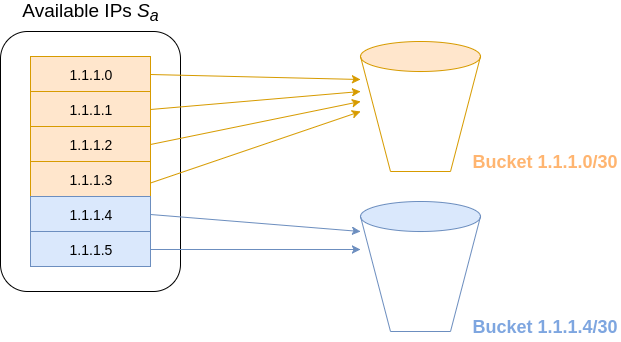
\includegraphics[width=0.7\textwidth]{renders/IpsByBucketSize4.png}
      \caption{Assigning IPs to Buckets with a Bucket Size of 4}
      \label{fig:exampleIpsByBucket4}
\end{figure}

As discussed, the bucket size will be an integral power of 2, but an important question is which integral power of 2. The algorithm starts by assigning the IPs to their buckets using a bucket size equal to the largest possible CIDR block that can be obtained for the given $t$. As discussed previously, this is the largest integral power of 2 that is less than or equal to $t$.

At this point, the algorithm begins to take shape. Consider the situation represented in \reffig{fig:exampleIpsByBucket4} along with a value of $t = 4$. The initial bucket size will be 4 and the presence of a filled bucket ($1.1.1.0/30$) indicates that a CIDR block of the bucket size can be created. Since the bucket size is equal to the desired number of IPs, the optimal choice is the $1.1.1.0/30$ block. The algorithm can return this block and it will be the optimum set of addresses to choose to minimize the number of CIDR entries required to represent the set of IP addresses.

Next consider the situation represented in \reffig{fig:exampleIpsByBucket4} along with a value of $t = 6$. The initial bucket size will still be 4 (as this is the largest integral power of 2 less than or equal to $t$). Thus, the algorithm will again detect that the $1.1.1.0/30$ bucket is full and select this block of four IPs. However the algorithm must return a total of $t = 6$ IPs and therefore must select a further 2 IPs. The algorithm accomplishes this by making a recursive call. By removing all of the (so far) selected IPs from the set of available IPs (forming $S_a'$, the \textit{available} set for the next call) and setting the new value of $t$ to be the remaining number of IPs required ($t'$ = 2), a recursive call will simply find the best set of IPs from what is left. This is shown in \reffig{fig:exampleIpsByBucket2} in which the recursive call would return $1.1.1.4/31$ as this bucket is full. The selected IPs from each recursive call are then unioned, returning the optimum set of IPs - $\{1.1.1.0/30,\enspace1.1.1.4/31\}$

\begin{figure}[H]
      \centering
      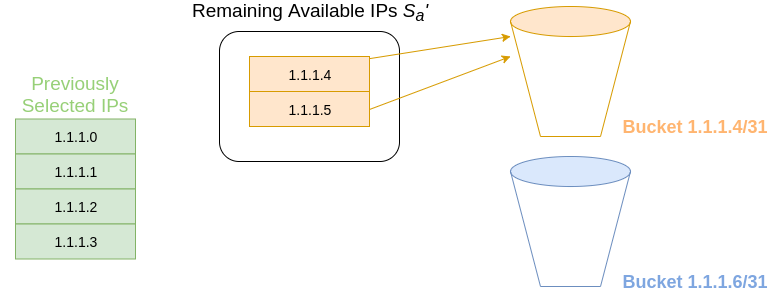
\includegraphics[width=0.8\textwidth]{renders/IpsByBucketSize2.png}
      \caption{Assigning Remaining IPs to Buckets with a Bucket Size of 2}
      \label{fig:exampleIpsByBucket2}
\end{figure}

In the case of $t = 7$, the algorithm would proceed as before, with one extra recursive call with $t = 1$. Assuming there were sufficient IPs available (the number of IPs in the diagrams were limited for brevity), the algorithm would have selected the same 6 IPs as before and the final call would be the trivial case of $t = 1$ in which a random IP can be selected. At each stage, the set of IPs returned from the recursive calls can then be unioned with the current call's chosen IPs, and the unioned set returned. 

The final possibility to consider is what should be done when no buckets are filled. In this case, the algorithm should not select any IPs at this bucket size. Instead, it should reduce the bucket size to the next highest integral power of 2 and recurse, setting $t$ equal to this reduced bucket size. However, there is another important step, the need for which is best illustrated with an example. A diagram of this situation is shown in \reffig{fig:ipAlgTrickyCodePath}

If the initial value for $t$ is 6, the initial bucket size will be 4. If no buckets of size 4 are filled, the algorithm will then recurse. Let this recursive call be denoted as $r_1'$, where $'$ indicates the depth of the recursion. Let the total number of IPs required for this recursive call $r_1'$ be denoted as $t_1'$. Thus, $t_1' = 2$ (the next largest integral power of 2 as discussed previously) and the set of available IPs is unchanged $S_{a_1}' = S_a$. Let the set of chosen IPs returned from $r_1'$ be denoted as $S_{c_1}'$.

The initial call required 6 IPs to be returned and $r_1'$ will return the 2 green IPs shown in \reffig{fig:ipAlgTrickyCodePath}, $\{1.1.1.0,\enspace1.1.1.1\}$. Thus, a second recursive call, $r_2'$ is required. This recursive call, $r_2'$ is \textbf{not} nested within the first recursive call $r_1'$, but rather is a sibling recursive call (it is at the same depth as $r_1'$).  Let the total number of IPs required for $r_2'$ be denoted as $t_2'$. $t_2'$ is calculated using the formula given in \refeq{eq:secondRecurseT2}. This is simply the remaining number of IPs that need to be chosen after the first recursive call. In this case, $t_2' = 6 - 2 = 4$. 

\begin{equation}\label{eq:secondRecurseT2}
t_2' = t - t_1'
\end{equation}

The set of available IPs that is used for $r_2'$, $S_{a_2}'$, is given by \refeq{eq:availableIpsSecondRecurse}. This is the initial set of all available IPs, with the IPs chosen from the first recursive call omitted. Let the set of IPs returned from $r_2'$ be denoted as $S_{c_2}'$.

\begin{equation}\label{eq:availableIpsSecondRecurse}
S_{a_2}' = S_a - S_{c_1}'
\end{equation}

\begin{figure}[H]
      \centering
      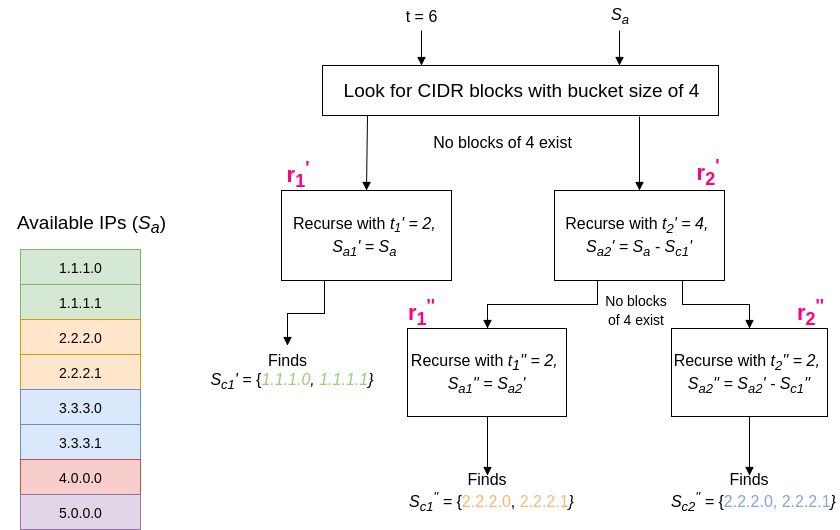
\includegraphics[width=\textwidth]{renders/IpAlgTrickyCodePath.png}
      \caption{Code Path When Algorithm Does Not Find Full Bucket}
      \label{fig:ipAlgTrickyCodePath}
\end{figure}

The second recursive call, $r_2'$ (as described above), will then look for IPs using a bucket size of 4. Again, none will be found. Thus, the algorithm will need to recurse again. Let this call be denoted $r_1''$. The bucket size for $r_1''$ will be 2 (the next highest integral power of 2). Thus, $r_1''$ will find the 2 IPs shown in orange in \reffig{fig:ipAlgTrickyCodePath}, $\{2.2.2.0,\enspace2.2.2.1\}$. However the second recursive call $r_2'$ required a total of 4 IPs and only 2 have been selected. Thus, just as in the first case, a sibling recursive call, $r_2''$ is required to choose the remaining IPs. Thus, $r_2''$ will require two more IPs to be chosen and will return the blue set of IPs shown in \reffig{fig:ipAlgTrickyCodePath}, $\{3.3.3.0,\enspace3.3.3.1\}$. The union of the results of $r_1''$ and $r_2''$ will be returned to $r_2'$ and will contain the required 4 IPs, $\{2.2.2.0/31,\enspace3.3.3.0/31\}$. Finally, the result of $r_1'$ and $r_2'$ will be unioned, returning the desired 6 IPs, $\{1.1.1.0/31,\enspace2.2.2.0/31,\enspace3.3.3.0/31\}$.

Now that all cases have been considered, the steps of the algorithm (for the simplified case of having no existing IPs) are shown below:
\begin{itemize}
\item{Set bucket size to the largest integral power of 2 that is less than or equal to $t$}
\item{Assign all available IPs into buckets using the calculated bucket size}
\item{If a bucket is full}
  \begin{itemize}
  \item{Add all the IPs in the bucket to the set of chosen IPs ($S_c$)}
  \item{Remove all the IPs in the bucket from the set of available IPs (forms $S_a'$)}
  \item{Calculate $t'$ as $t - bucketSize$}
  \item{Recurse using $S_a'$ and $t'$ (if necessary)}
  \end{itemize}
\item{Otherwise}
  \begin{itemize}
  \item{Recurse ($r_1'$) using next biggest integral power of 2 and the initial set of available IPs}
  \item{Recurse again ($r_2'$) using the remaining number of IPs required and the set of available IPs, excluding those returned from $r_1'$ ($S_{c_1}'$)}
  \item{Return the union of the results of the two recursive calls.}
  \end{itemize}
\end{itemize}

\subsection{Extending the Algorithm to Support Existing IPs}
Now that a solution to the simplified problem where $S_e = \{\}$ has been formed, the more complex initial problem could now be tackled. However upon closer inspection, there is only one extra point to consider when the set of existing IPs is non empty: \textbf{the final set must be a super set of the set of existing IPs}. 

The extended algorithm's parameters are changed to the following to aid in the recursion:

\begin{itemize}
\item{A list of available IPs - $S_a$}
\item{A list of existing IPs - $S_e$}
\item{The total number of IPs desired - $t$}
\item{The bucket size to use - $b$}
\end{itemize}

The main changes to the algorithm are the following:

\begin{itemize}
  \item{Assign the existing IPs ($S_e$) to buckets using the provided bucket size}
  \item{Assign the available IPs ($S_a$) to separate buckets using the provided bucket size}
  \item{For each of the \textit{existing} IP buckets $S_{e_i}$}
      \begin{itemize}
      \item{Calculate $b^*_i$, the number of IPs required to fill the bucket (\refeq{eq:ipsToFillBucket})}
      \item{If the number of IPs in the corresponding \textit{available} IP bucket ($S_{a_i}$) equals $b^*_i$, the union of the two buckets creates a CIDR block and should be added to the currently chosen set of IPs ($S_c$), as long as it doesn't cause $|S_c|$ to become larger than the total number of desired IPs, $t$}
      \item{If $|S_c|$ is now equal to $t$ (the total number of IPs required), $S_c$ can be returned.}
      \item{Otherwise, recurse (see below)}
      \end{itemize}
\end{itemize}


\begin{equation}\label{eq:ipsToFillBucket}
b^*_i= b-|S_{e_i}|
\end{equation}


This shows that the only logical change is that the number of IPs required to \textit{fill the existing IP buckets} should be examined, rather than searching for full buckets from the available pool. 

As with the simplified case, this method may require some recursion after the above steps. The recursive call in this case is actually simpler, but depends on the current state of the algorithm. As previously mentioned, all the IPs in the existing set should be contained in the final set. If the algorithm reaches a state where all the existing IPs have been used, but there is still a number of IPs to be selected, the algorithm can simply fallback to the previous case where $S_e = \{\}$. 

Otherwise, the algorithm recurses using the remaining available IPs, the remaining \textit{required} IPs (this is the set of existing IPs that have not yet been chosen), the remaining number of IPs to be chosen and the next bucket size to use which is the next largest integral power of 2.

Consider the following example as shown in \reffig{fig:ipsByBucketExisting4}.
\begin{itemize}
\item{$S_e = \{1.1.1.0,\enspace2.2.2.0\}$}
\item{$S_a = \{1.1.1.1,\enspace1.1.1.2,\enspace1.1.1.3,\enspace2.2.2.1,\enspace2.2.2.2\}$}
\item{$t = 7$}
\end{itemize}

As $t = 7$, the initial bucket size $b$ would be 4 and the IPs would be assigned to buckets as shown in \reffig{fig:ipsByBucketExisting4}

The algorithm would then proceed in the following manner:
\begin{itemize}
\item{Examine each existing bucket ($S_{e_i}$) and the corresponding available bucket ($S_{a_i}$)}
\begin{itemize}
\item{Calculate $b_i^*$ for $1.1.1.0/30$ as per \refeq{eq:ipsToFillBucket}, yielding 3}
\item{Add $1.1.1.0/30$ to $S_c$ as $b^*_i = |S_{a_i}| = 3$}
\end{itemize}
\begin{itemize}
\item{Calculate $b_i^*$ for $2.2.2.0/30$ as per \refeq{eq:ipsToFillBucket}, also yielding 3}
\item{Skip $2.2.2.0/30$ as $b^*_i > |S_{a_i}|$ ($3 > 2$)}   
\end{itemize}
\end{itemize}

\begin{figure}[H]
      \centering
      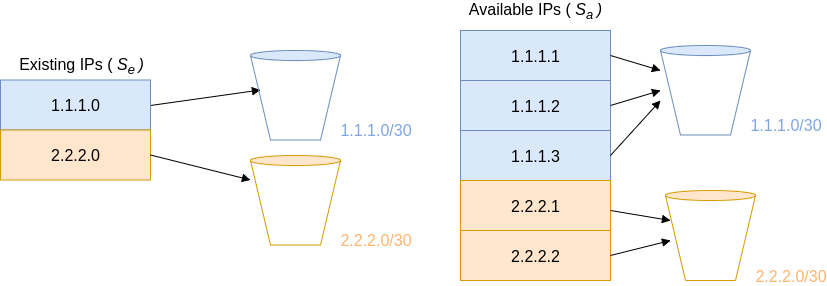
\includegraphics[width=0.8\textwidth]{renders/IpsByBucketSize4Existing.png}
      \caption{Available and Existing IPs Assigned to Buckets of Size 4}
      \label{fig:ipsByBucketExisting4}
\end{figure}

Since the total number of IPs required was $t = 7$ and only 4 IPs have been selected, a recursive call is required. As there are still some existing IPs that have not been included, a recursive call is made with the following parameters:
\begin{itemize}
\item{$S'_e = \{2.2.2.0\}$ - the remaining \textit{required} IPs that have not yet been chosen}
\item{$S'_a = \{2.2.2.1,\enspace2.2.2.2\}$ - the remaining \textit{available} IPs}
\item{$t' = 3$ - the remaining \textit{number} of IPs to be selected}
\item{$b' = 2$ - the bucket size should be the next largest integral power of 2 (was 4)}
\end{itemize}

Thus, the IPs will be assigned to buckets of size 2, as shown in \reffig{fig:ipsByBucketExisting2}.

The algorithm will then proceed as follows:
\begin{itemize}
\item{Examine each existing bucket ($S_{e_i}'$) and the corresponding available bucket ($S_{a_i}'$)}
\begin{itemize}
\item{Calculate $b*'_i$ for $2.2.2.0/31$ as per \refeq{eq:ipsToFillBucket}, yielding 1}
\item{Add $2.2.2.0/31$ to $S_c'$ as $b*'_i = |S'_{a_i}| = 1$} 
\item{Skip $2.2.2.2/31$ as $b*'_i > |S'_{a_i}| (2 > 1)$}
\end{itemize}
\end{itemize}

\begin{figure}[H]
      \centering
      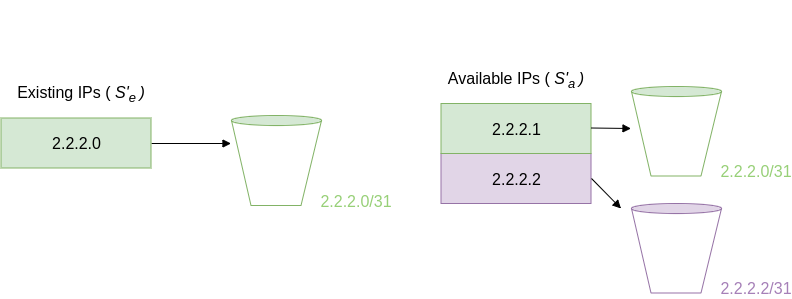
\includegraphics[width=0.8\textwidth]{renders/IpsByBucketSize2Existing.png}
      \caption{Remaining Available and Existing IPs Assigned to Buckets of Size 2}
      \label{fig:ipsByBucketExisting2}
\end{figure}

Finally, since a total of 7 IPs were required and 6 have now been selected, a final recursive call is required. However all the existing IPs have now been chosen, meaning the existing IPs argument for the next recursive call will empty. This means the algorithm falls back to the simple case as described earlier and will choose a random final IP ($2.2.2.2$ in this case). 

There are two enhancements that can be made to the algorithm at this point.

\begin{enumerate}
\item{A better method for choosing a \textbf{single} IP from the available IP pool. This shouldn't be done randomly as this could result in large CIDR blocks contained in the available IP pool being broken up unnecessarily. This is described in \refapp{appendix:smartSingleIP}.}
\item{In the case where the existing set of IPs ($S_e$) is non empty, the previously described method of choosing the highest integral power of 2 that is less than or equal to $t$ for the initial bucket size is not ideal. Given a set of 2 IPs and requiring a total of 4 IPs, the approach would suggest starting with a bucket size of 4. However unless the existing IPs themselves are contiguous, there is no possibility of forming a CIDR block of size 4. This is described in detail in \refapp{appendix:smartInitBucket}.}
\end{enumerate}

Finally, the entire source code for the algorithm can be found in \refapp{appendix:cidrMinSource}

\break

\subsection{Unit Testing the Algorithm}
The final step in the development was to write extensive unit tests to ensure the algorithm operates as expected. Unit testing is a critical part of the software development process at HubSpot and engineers are always encouraged to write code which is as unit testable as possible. As the code is essentially a number of static utility functions, unit testing is quite simple and does not require mocking any complex objects.  

The initial task was to come up with an example state to test the algorithm with. The example state contains the set of available IP addresses $S_a$ and the set of existing IP addresses $S_e$. These should be chosen in such a way that all code paths of the algorithm are seen at some point or another when running the tests. This requires some consideration as for what is contained in $S_a$ and $S_e$, as well as the total number of IPs required, $t$, for each of the test cases.

As a starting point, the following sets of IPs were chosen for the default state (this can be changed on a per test basis of course):

\begin{equation}\label{eq:initialState}
\begin{gathered}
S_a = \{1.1.1.2,\enspace1.1.1.3,\enspace1.1.1.4,\enspace1.1.1.5,\enspace1.1.1.6,\enspace1.1.1.7,\enspace1.1.1.8,\enspace1.1.1.9\} \\
S_e = \{1.1.1.0,\enspace1.1.1.1\}
\end{gathered}
\end{equation}

Initially however, tests were written for the simplified case where $S_e = \{\}$. The following tests were then implemented:

\begin{itemize}
\item{The algorithm should choose contiguous blocks when available}
      \begin{itemize}
      \item{This was tested by simply requesting that 4 IPs be selected from $S_a$ and ensuring that the resulting set was $\{1.1.1.4/30\}$.}
      \end{itemize}
\item{The algorithm should find contiguous blocks of IPs when a single IP will be left over}
      \begin{itemize}
      \item{This was tested by requesting that 5 IPs be selected from $S_a$}
      \item{The resulting set should contain the block of 4 IP addresses ($1.1.1.4/30$) and a single other IP}
      \item{This test was added to ensure that the algorithm still selected a block of four instead of trying to find several blocks of 2}
      \end{itemize}
\item{The algorithm should find contiguous IPs recursively}
      \begin{itemize}
      \item{This was tested by requesting that 6 IPs be selected from $S_a$}
      \item{The resulting set should contain the block of 4 IP addresses ($1.1.1.4/30$) as before, but should also select the $1.1.1.2/31$ block for the remaining 2 IP addresses}
      \item{This test was sufficient to assume the algorithm would recursively select CIDR blocks at lower block sizes when available}
      \end{itemize}
\item{The algorithm should always return the correct number of IP addresses}
      \begin{itemize}
      \item{This test was implemented by repeatedly invoking the algorithm with $t$ running from $1$ to $|S_a|$ and ensuring $|S_c| = t \enspace \forall \enspace t$}
      \end{itemize}
\end{itemize}

These tests were sufficient for the simple case where $S_e = \{\}$ and the algorithm was then tested using the more complex case. The following tests were implemented in order to ensure correctness of the algorithm:

\begin{itemize}
\item{The algorithm should find contiguous blocks when provided with existing IP addresses}
      \begin{itemize}
      \item{This was tested by requesting a total of 4 IPs, given the default state as described in \refeq{eq:initialState}}
      \item{The algorithm should then select $\{1.1.1.2/31\}$} so that when unioned with $S_e = \{1.1.1.0/31\}$, the CIDR block $\{1.1.1.0/30\}$  is formed 
      \end{itemize}
\item{The algorithm should always return the correct number of IPs and contain all the existing IPs}
      \begin{itemize}
      \item{This test was an important test as the algorithm would be useless if it minimized CIDR blocks but didn't guarantee that all of the existing IPs would be present in the resulting set}
      \item{This test was implemented by allowing a variable $i$ to take on values from $1$ to $|S_a|$ and by setting $t = |S_e| + i$.}
      \item{This essentially repeatedly runs the algorithm, requesting each possible value from the minimum number of new IPs (1), to the maximum number of new IPs (the number of available IPs)}
      \item{At each iteration, the returned set was checked to ensure the correct number of IPs was returned and that all of the existing IPs were contained in that set.}
      \end{itemize}
\item{The algorithm was also tested to ensure it would look for contiguous blocks both above and below (in the IP address space) the existing IPs provided in order to try and find CIDR blocks}
      \begin{itemize}
      \item{This was tested by requesting a total of 2 IPs and setting $S_e = \{1.1.1.3\}$}
      \item{This tested that the algorithm would find CIDR blocks below the existing IPs provided}
      \item{The algorithm should return $1.1.1.2/31$, indicating it correctly searches below the provided existing IPs}
      \item{A similar test was written where $S_e = {1.1.1.2}$ and the algorithm correctly returned $1.1.1.2/31$ indicating that it also looks above the provided existing IP addresses for CIDR blocks}
      \end{itemize}
\item{The algorithm should find CIDR blocks with existing IP addresses that cause a single IP to be left over}
      \begin{itemize}
      \item{This was tested by requesting a total of 9 IPs using the default state as shown in \refeq{eq:initialState}}
      \item{The resulting set should contain the CIDR block of 8 IPs ($1.1.1.0/29$) and the remaining extra IP ($1.1.1.9$)}
      \end{itemize}
\item{The algorithm should return already grouped existing IPs}
      \begin{itemize}
      \item{It is essentially impossible to break up a CIDR block contained inside the set of existing IP addresses, but this test was added to ensure the algorithm correctly identified existing CIDR blocks appropriately.}
      \item{A set of existing IPs $S_e = \{2.2.2.0/31\}$ was used along with the available set of IPs listed in \refeq{eq:initialState} and a total of 4 IPs were requested.}
      \item{The algorithm correctly returned the existing CIDR block as well as another CIDR block of size 2, yielding $\{1.1.1.2/31,\enspace2.2.2.0/31\}$}
      \item{This ensured the algorithm selected the existing block of 2 as well as another block of 2, instead of selecting a block of 4 by excluding existing IPs}
      \end{itemize}
\item{The algorithm should handle existing IPs which don't contribute to any CIDR blocks and should fill the remaining number of IPs required with the best CIDR block from the available set of IPs}
      \begin{itemize}
      \item{This was tested by setting $S_e = \{2.2.2.0,\enspace3.3.3.0,\enspace4.4.4.0\}$}, using the set of available IPs shown in \refeq{eq:initialState} and requesting 5 IPs.
      \item{The algorithm should then return the three existing IPs along with a CIDR block of size 2 from the set of available IPs}
      \end{itemize}
\end{itemize}

These tests provided a sufficient amount of coverage to provide confidence in the algorithm and its implementation. Several other tests were implemented which were less specific to the algorithm (such as ensuring user input was validated). The algorithm has been running in a production environment for over 3 months and has helped automate an important step that was previously being performed manually by a support team at HubSpot.   

\section{Abstracting Upstream Email Sending to Kafka}
While discussing Kafka in \refsec{sec:kafka}, an idealized case of having all emails that need to be sent through HubSpot simply placed on a Kafka topic was shown. This functionality is supported for emails that can be sent through HubSpot's internal Mail Transfer Agent (MTA) (see \refsec{sec:emailSendingInfra} for more details), but is not supported for emails using other third party MTAs. The reason for this was HubSpot's email marketing was initially built using third party MTAs, prior to the development of the internal MTA. Prior to this task, email sent through third party MTAs was done \textit{in-process}, inside of an upstream email team's deployable, as all of this code was written prior to the formation of the \team{} team. This code is entirely to do with email sending and thus should certainly be owned and controlled by the \team{} team. It also adds a considerable amount of latency to the upstream email team's code, as they must wait for the results of email sends. 

The main goal of this task was to decouple the email sending code from the upstream teams deployable. Kafka was the perfect choice to use as the interface between the two teams and the desired setup was for the upstream team to produce the emails to be sent to a given Kafka topic, for those emails to be sent by the \team{} team's Kafka consumers and for the results of the email send to be produced back to the upstream email team through a second Kafka topic.

The major difficulty associated with rewriting the code in this way was that the results of the email send were no longer obtainable in-process of the upstream teams deployable. The email sending would essentially happen asynchronously and the results would be present in a \textbf{different} deployable. Ultimately this is the exact behavior that is desired as the process producing these emails to Kafka should be able to \textit{"fire and forget"} - once it has produced the email to Kafka, it has done its job.

The main difficulty associated with this task was implementing the solution in a \textit{backwards compatible} way. All of HubSpot's outgoing marketing email would be run through this new code path. Thus, it must be rolled out extremely slowly and carefully. This meant the code changes must be made in such a way that either the old in-process email sending, or the new Kafka email sending could be used. 

This task was essentially two tasks which were entirely dependent on one and other. One of these tasks was creating the infrastructure required on the \team{} team's side of things and the other was making use of this infrastructure on the upstream email team's side of things.
\break

\subsection{The \team{} Team's Side}
This task required the creation of an entirely new project owned by the \team{} team. This project would now contain all the code required for sending the emails to both the internal MTA and the third party MTAs. This required substantial research into setting up and configuring Kafka and setting up a project on the HubSpot stack. 

As discussed, all changes had to be backwards compatible. This was achieved by writing a new higher level abstraction of a class which sends emails. To the upstream team, they would simply obtain a reference to an object which had a \java{produceEmailRequest} method. Under the hood, there were several implementations of an interface which contained this method. One of these implementations provided access to the old in-process email senders, while the other implementations provided access to the new Kafka producers which would produce these emails to the new Kafka topic. This abstraction was provided to the upstream team, allowing the \team{} team to control \textit{under what circumstances} and \textit{when} the new Kafka sending pipeline could be used. For example, the Kafka senders could be used a configurable number of times per minute, for particular types of email sends, or disabled entirely.

This extra consideration and layer of abstraction was key in providing a mechanism for safely rolling out changes which could potentially break \textbf{every} email that was to be sent through HubSpot.

\subsection{The Upstream Email Team's Side}
The upstream email team in this case were the team responsible for managing all the data generated around an email to be sent. In this circumstance, their main task was performing all the required work that was to be done post send attempt. This included writing the email to a variety of places, producing events which lead to customer billing, tracking the number of sends a particular customer had made and many others. 

The main issue at this point was some of this \textit{post-send} logic required the \textbf{result} of the email send. However as the main purpose of this task was to decouple the email send from their process and reduce latency, by definition, the results of email sends were no longer available. This required careful splitting out of the \textit{post-send} logic into what could be performed in-process and what could not. Any of the logic which was entirely dependent on the result of the email send had to be moved into a Kafka consumer, listening to the results of the email sends, which were produced by the \team{} team's Kafka consumers who were responsible for sending the email.

Though the task may seem trivial, this was actually one of the most difficult tasks undertaken throughout the course of the internship. A monumental amount of research and consideration was required in order to ensure all edge cases were covered and that the new Kafka sending pipeline would be stable. As discussed, every marketing email sent through HubSpot would run through this code and this code was also responsible for billing customers, so any bugs could have proved extremely costly.


\chapter{Conclusion}
In conclusion, the internship provided a fantastic insight into how software is developed in an enterprise environment and provided ample opportunity to learn new concepts and extend knowledge on previously studied topics. 

Over the course of the internship, experience was gained working with a variety of new and exciting technologies such as Kafka (\refsec{sec:kafka}) and Hadoop (\refsec{sec:hadoop}). Knowledge gained from previous modules of the course on fundamental computer science principles, problems and techniques (for example immutability, dependency injection, databases and distributed systems) was put into practice and used to deliver industry standard, well tested software that is used millions of times per day in a production environment.

The internship also provided an opportunity to practice and improve upon softer skills such as time management, time estimation for software development tasks, hosting and contributing to meetings with other engineers and reviewing code submitted by teammates. Although modules aiding in developing these fundamental industry skills are available throughout the MAI program, having the chance to use these skills on a daily basis provides an excellent means of improving these skills in a real enterprise environment.


\bibliographystyle{unsrtnat}
\bibliography{bibliography}

% Prepend App. to chapter headings
\titleformat{\chapter}[block] 
{\normalfont\LARGE\bfseries}{App. \thechapter}{0.6cm}{} 
\begin{appendices}

\chapter{Source Code for DNS Management System}
\label{appendix:dnsManagement}
\lstinputlisting[
  caption={The \java{DnsRecordBuilder} Interface},
  label={lst:dnsRecordBuilder},
  style=javaStyle
  ]{code/tasks_undertaken/dns_management/DnsRecordBuilder.java}

\lstinputlisting[
  caption={Apply \java{DnsRecordBuilder}s and Find Records That Need Updating.},
  label={lst:recordBuilderApplier},
  style=javaStyle
  ]{code/tasks_undertaken/dns_management/DnsRecordBuilderApplier.java}

\lstinputlisting[
  caption={A Simplified DNS Sync Job Implementation},
  label={lst:dnsSyncJob},
  style=javaStyle
  ]{code/tasks_undertaken/dns_management/DnsSyncJob.java}

\chapter{CIDR Min. Algorithm - Single IP Choice}
\label{appendix:smartSingleIP}
When selecting a single IP from the available pool, ideally, the algorithm should choose an \textit{awkward} IP that does not have any free neighboring IPs. Otherwise, the algorithm may break up valuable CIDR blocks by choosing randomly. 

This enhancement to the algorithm was added by examining the set of available IPs and attempting to find a bucket containing a single IP. A list of IPs denoted as \java{remainingIps} is initialized to contain the same IPs as the \java{availableIps} set. An initial bucket size was defined and the available IPs were assigned to buckets at this size. The bucket with the smallest number of IPs was then selected. If the number of IPs in this bucket was 1, this IP would be returned. Otherwise, the \java{remainingIps} list was set to the IPs in this bucket and the process would be repeated with a smaller bucket size. 

This allows IPs that \textit{may} form CIDR blocks to be kept available for cases when more than 1 IP is requested. 

The code for the function is shown in \refcode{lst:singleAwkIp}

\textbf{Note for the sake of the report, the size of the bucket was used for explanatory purposes. However the code makes frequent use of the number of host bits. These are related through \refeq{eq:bucketSizeHostBits1}}

\begin{equation}\label{eq:bucketSizeHostBits1}
bucketSize = 2^{numHostBits}
\end{equation}
\vfill

\lstinputlisting[
  caption={Finding a Single Awkward IP},
  label={lst:singleAwkIp},
  style=javaStyle
  ]{code/appendix/SingleIp.java}


\chapter{CIDR Min. Algorithm - Initial Bucket Size}
\label{appendix:smartInitBucket}
The previously described method for choosing the initial bucket size was choosing the highest integral power of 2 that is less than or equal to $t$. This method only makes sense for the case where $S_e = \{\}$. 

For example, given $S_e = \{1.1.1.0,\enspace2.2.2.0\}$ and $t = 4$ the algorithm must choose two IPs ($n = 2$). The described method would suggest starting with a bucket size of $b=4$. However it would be impossible to generate a CIDR block of size 4 given the existing IPs and a choice of only two IPs, \textbf{regardless of the available IPs}. 

This extension is handled by a separate function which is called prior to starting the algorithm, to determine the appropriate starting bucket size. This function only requires the total number of IPs desired ($t$) and the existing set of IPs ($S_e$) as parameters. 

The function starts by assigning IPs to buckets using the largest integral power of 2 less than or equal to $t$ rule. It then calculates $n$ (the number of IPs that need to be chosen from the available pool) and checks if any of the existing buckets require \textbf{$n$ or less} IPs to be filled. As only $n$ or less IPs can be selected, if no buckets can be \textit{filled} by selecting $n$ or less IPs, there is no possibility of creating CIDR blocks at this bucket size. This is done without considering the available IPs. Thus, even if a bucket \textit{could} be filled by choosing $n$ IPs, it may not be. If no buckets can be filled choosing $n$ or less IPs, the loop continues, checking the next largest bucket size. Otherwise, the function returns the current bucket size.

\textbf{Note for the sake of the report, the size of the bucket was used for explanatory purposes. However the code makes frequent use of the number of host bits. These are related through \refeq{eq:bucketSizeHostBits2}}

\begin{equation}\label{eq:bucketSizeHostBits2}
bucketSize = 2^{numHostBits}
\end{equation}

\vfill
\lstinputlisting[
  caption={Choosing the Initial Bucket Size},
  label={lst:initBucketSize},
  style=javaStyle
  ]{code/appendix/InitialBucketSize.java}




\chapter{CIDR Min. Algorithm - Source Code}
\label{appendix:cidrMinSource}
\lstinputlisting[
  caption={CIDR Minimization Algorithm Source Code},
  label={lst:cidrMinAlgCode},
  style=javaStyle
  ]{code/appendix/IpAlg.java}
\end{appendices}

\end{document}